%
%  THESISBOEK
%
%  Dit bestand zorgt voor algemene (layout)definities, en groepeert de
%  afzonderlijke LaTeX-files tot een geheel.
%
%  @author Erwin Six, David De Reu, Brecht Vermeulen
%

\documentclass[11pt,a4paper,oneside,notitlepage]{book}
\usepackage[english,dutch]{babel}
\usepackage[intoc]{nomencl}
\makenomenclature
\renewcommand{\nomname}{Lijst van gebruikte afkortingen}
\usepackage{wrapfig}
\makeindex

\usepackage{eurosym}
\usepackage[font=small,format=plain,labelfont=bf,up,textfont=it,up]{caption}
\usepackage{subcaption}
\usepackage{listings}
\usepackage{color}
\usepackage{xcolor}
\usepackage{caption}

\DeclareCaptionFont{white}{\color{white}}
\DeclareCaptionFormat{listing}{\colorbox{gray}{\parbox{\textwidth}{#1#2#3}}}
\captionsetup[lstlisting]{format=listing,labelfont=white,textfont=white}

% marges aanpassen
% (opmerking: moet *voor* inclusie van fancyhdr package komen)
\setlength{\hoffset}{-1in}
\setlength{\voffset}{-1in}
\setlength{\topmargin}{2cm}
\setlength{\headheight}{0.5cm}
\setlength{\headsep}{1cm}
\setlength{\oddsidemargin}{3.5cm}
\setlength{\evensidemargin}{3.5cm}
\setlength{\textwidth}{16cm}
\setlength{\textheight}{23.3cm}
\setlength{\footskip}{1.5cm}

\usepackage{fancyhdr}
\usepackage{graphicx}
% \usepackage[colorlinks]{hyperref}

\pagestyle{fancy}

\renewcommand{\chaptermark}[1]{\markright{\MakeUppercase{#1}}}
\renewcommand{\sectionmark}[1]{\markright{\thesection~#1}}

\newcommand{\headerfmt}[1]{\textsl{\textsf{#1}}}
\newcommand{\headerfmtpage}[1]{\textsf{#1}}

\fancyhf{}
\fancyhead[LE,RO]{\headerfmtpage{\thepage}}
\fancyhead[LO]{\headerfmt{\rightmark}}
\fancyhead[RE]{\headerfmt{\leftmark}}
\renewcommand{\headrulewidth}{0.5pt}
\renewcommand{\footrulewidth}{0pt}

\fancypagestyle{plain}{ % eerste bladzijde van een hoofdstuk
  \fancyhf{}
  \fancyhead[LE,RO]{\headerfmtpage{\thepage}}
  \fancyhead[LO]{\headerfmt{\rightmark}}
  \fancyhead[RE]{\headerfmt{\leftmark}}
  \renewcommand{\headrulewidth}{0.5pt}
  \renewcommand{\footrulewidth}{0pt}
}

% anderhalve interlinie (opm: titelblad gaat uit van 1.5)
\renewcommand{\baselinestretch}{1.5}

% indien LaTeX niet goed splitst, neem je woord hierin op, of evt om splitsen 
% te voorkomen
\hyphenation{ditmagnooitgesplitstworden dit-woord-splitst-hier}

\begin{document}

% titelblad (voor kaft)
%  Titelblad

% Opmerking: gaat uit van een \baselinestretch waarde van 1.5 (die moet
% ingesteld worden voor het begin van de document environment)

\begin{titlepage}

\setlength{\hoffset}{-1in}
\setlength{\voffset}{-1in}
\setlength{\topmargin}{1.5cm}
\setlength{\headheight}{0.5cm}
\setlength{\headsep}{1cm}
\setlength{\oddsidemargin}{3cm}
\setlength{\evensidemargin}{3cm}
\setlength{\footskip}{1.5cm}
\enlargethispage{1cm}
% \textwidth en \textheight hier aanpassen blijkt niet te werken

\fontsize{12pt}{14pt}
\selectfont

\begin{center}


\includegraphics[height=4cm]{fig/hogentLogo}

\vspace{0.5cm}

Geassocieerde Faculteit Toegepaste Ingenieurswetenschappen\\
Vakgroep Informatica

\vspace{3.5cm}

\fontseries{bx}
\fontsize{17.28pt}{21pt}
\selectfont

Internet of Things: Integratie in Drupal

\fontseries{m}
\fontsize{12pt}{14pt}
\selectfont

\vspace{.6cm}

door 

\vspace{.4cm}

Kobe WRIGHT\\
Stef DE WAELE

\vspace{3.5cm}

Promotoren: dr.~ir.~J.~HOEBEKE, prof.~dr.~ir.~I.~MOERMAN, dr.~ir.~P.~SIMOENS\\
Begeleiders: ing.~J.~ROSSEY, ir.~F.~VAN DEN ABEELE\\

\vspace{2cm}

Masterproef voorgedragen tot het behalen van het diploma van\\
Master in de industri\"{e}le wetenschappen: informatica

\vspace{1cm}

Academiejaar 2012--2013

\end{center}
\end{titlepage}


% lege pagina (!!)
\newpage
\thispagestyle{empty}
\mbox{}

% titelblad (!!)
%  Titelblad

% Opmerking: gaat uit van een \baselinestretch waarde van 1.5 (die moet
% ingesteld worden voor het begin van de document environment)

\begin{titlepage}

\setlength{\hoffset}{-1in}
\setlength{\voffset}{-1in}
\setlength{\topmargin}{1.5cm}
\setlength{\headheight}{0.5cm}
\setlength{\headsep}{1cm}
\setlength{\oddsidemargin}{3cm}
\setlength{\evensidemargin}{3cm}
\setlength{\footskip}{1.5cm}
\enlargethispage{1cm}
% \textwidth en \textheight hier aanpassen blijkt niet te werken

\fontsize{12pt}{14pt}
\selectfont

\begin{center}


\includegraphics[height=4cm]{fig/hogentLogo}

\vspace{0.5cm}

Geassocieerde Faculteit Toegepaste Ingenieurswetenschappen\\
Vakgroep Informatica

\vspace{3.5cm}

\fontseries{bx}
\fontsize{17.28pt}{21pt}
\selectfont

Internet of Things: Integratie in Drupal

\fontseries{m}
\fontsize{12pt}{14pt}
\selectfont

\vspace{.6cm}

door 

\vspace{.4cm}

Kobe WRIGHT\\
Stef DE WAELE

\vspace{3.5cm}

Promotoren: dr.~ir.~J.~HOEBEKE, prof.~dr.~ir.~I.~MOERMAN, dr.~ir.~P.~SIMOENS\\
Begeleiders: ing.~J.~ROSSEY, ir.~F.~VAN DEN ABEELE\\

\vspace{2cm}

Masterproef voorgedragen tot het behalen van het diploma van\\
Master in de industri\"{e}le wetenschappen: informatica

\vspace{1cm}

Academiejaar 2012--2013

\end{center}
\end{titlepage}


% geen paginanummering tot we aan de inhoudsopgave komen
\pagestyle{empty}

% voorwoord met dankwoord en toelating tot bruikleen (ondertekend)
%  Voorwoord (dankwoord) en toelating tot bruikleen

\newpage

\noindent \textbf{\huge Voorwoord}

\vspace{1.5cm}

\noindent
Graag bedanken we onze begeleiders Jen Rossey en Floris Van Den Abeele. Zij hebben ons doorheen de masterproef meermaals het licht getoond wanneer we in lastige situaties verzeild raakten. Ook willen we onze interne promotor Pieter Simoens bedanken. We waarderen zijn hulp enorm bij het schrijven van deze scriptie en het opstellen van onze poster. Verder bedanken we onze externe promotoren, Jeroen Hoebeke en Ingrid Moerman. Het zijn zij die ons in de eerste plaats deze masterproef hebben aangeboden. \\
Deze masterproef werd mogelijk gemaakt door de onderzoeksgroep iMinds. De accomodatie en het gebruik van de apparatuur hebben een positieve invloed gehad op het resultaat. We hopen dan ook dat deze scriptie een uitgangspunt mag zijn voor verdere ontwikkelingen.\\
Tot slot willen we graag alle andere mensen bedanken die ook rechtstreeks of onrechtstreeks een bijdrage geleverd hebben tot het realiseren van deze masterproef.

\addvspace{4cm}

\noindent Kobe Wright \& Stef De Waele, mei 2013\newpage

\noindent \textbf{\huge Toelating tot bruikleen}

\vspace{1.5cm}

\noindent
``De auteur geeft de toelating deze scriptie voor consultatie beschikbaar
te stellen en delen van de scriptie te kopi\"eren voor persoonlijk
gebruik.\\
Elk ander gebruik valt onder de beperkingen van het auteursrecht,
in het bijzonder met betrekking tot de verplichting de bron uitdrukkelijk
te vermelden bij het aanhalen van resultaten uit deze scriptie.''

\addvspace{4cm}

\noindent Kobe Wright \& Stef De Waele, mei 2013


% overzicht
%  Overzichtsbladzijde met samenvatting

\newpage

{
\setlength{\baselineskip}{14pt}
\setlength{\parindent}{0pt}
\setlength{\parskip}{8pt}

\begin{center}

\noindent \textbf{\huge
Internet of Things: Integratie in Drupal
}

door 

Kobe WRIGHT\\
Stef DE WAELE

Masterproef voorgedragen tot het behalen van het diploma van\\
Master in de industri\"{e}le wetenschappen: informatica

Academiejaar 2012--2013

Promotoren: dr.~ir.~J.~HOEBEKE, prof.~dr.~ir.~I.~MOERMAN, dr.~ir.~P.~SIMOENS\\
Begeleiders: ing.~J.~ROSSEY, ir.~F.~VAN DEN ABEELE\\

Geassocieerde Faculteit Toegepaste Ingenieurswetenschappen\\
Hogeschool Gent

Vakgroep Informatica

\end{center}

\section*{Samenvatting}

% TODO: samenvatting

Het \textit{Internet of Things} wordt steeds belangrijker. Bij dit concept staat het idee dat verscheidene soorten apparaten rechtstreeks of onrechtstreeks met het internet verbonden worden centraal. Het biedt de mogelijkheid deze apparaten van op afstand te observeren en te besturen op een gemakkelijke en dynamische manier. Deze apparaten zijn in werkelijkheid vaak beperkt in mate van energieverbruik en geheugen. Vaak is het netwerk waarmee ze verbonden zijn eveneens beperkt waardoor beperkte bandbreedte en onbetrouwbare verbindingen niet zeldzaam zijn.

Het doel van deze masterproef bestaat erin een Drupalmodule te ontwikkelen die het mogelijk maakt op een gebruiksvriendelijke en dynamische manier sensordata op te vragen en sensoren te configureren. Hierbij moet rekening gehouden worden met de beperkte mogelijkheden van zowel het netwerk als van de aangesloten apparaten. Ook moet de module ruimte laten voor uitbreidingen en moeten de recente mogelijkheden van Drupal 7 benut worden met een oog op de aangeboden functionaliteit van Drupal 8. Enige commentaar in code mag dan ook niet ontbreken.

Om de communicatie tussen de devices over het netwerk te waarborgen is HTTP te zwaar. Daarom wordt er gebruik gemaakt van het minder zware CoAP. In ruil voor de betrouwbaarheid en robuustheid van HTTP biedt CoAP een minimale overhead, een hoge mate van simpliciteit en features die zich niet beperken tot de observe-functionaliteit en blockwise transfer.

Als resultaat bieden we twee Drupalmodules aan. De CoAP-\textit{library}- en de CoAP-sensormodule. De CoAP-\textit{library} verzorgt alle communicatie tussen clients en servers op een netwerk door middel van native CoAP. Deze module heeft op zich weinig te bieden aan de doorsnee Drupalgebruiker en heeft enkel als doel een CoAP API aan te bieden aan Drupalontwikkelaars. Deze \textit{stand-alone} module kan ook gebruikt worden in andere projecten waar een PHP-implementatie van CoAP voor Drupal vereist is. De CoAP-sensormodule maakt gebruik van de CoAP-\textit{library} en biedt de gebruiksvriendelijke interface aan waarmee Drupalgebruikers sensoren kunnen beheren.

\section*{Abstract}
The Internet of Things is increasing in importance every day. The Central idea in this concept is that multiple kinds of devices are connected to the internet in a direct or indirect way. It offers the possibility to observe or configure these devices in a user-friendly and dynamic way. These devices are more often than not constrained in both energy supply and memory. Most of the time the network on which they are located is also constrained. Which results in low bandwidth and unreliable connections. 

The aim of this thesis is to develop a Drupal module which allows a user-friendly and dynamic way to collect sensor data and to configure sensors. It must be taken into account that the devices and the network which they are connected to, are constrained. The module also needs to leave room for expansions and needs to take advantage from the recent possibilities from Drupal 7 while not neglecting the functionalities of Drupal 8. Therefore comments in the code should not be absent. 

HTTP is too heavy to make the communication between the devices possible. Because of this, CoAP is used instead, which is a lightweight protocol. CoAP exchanges the reliability and robustness from HTTP for a minimal overhead, a simplified design and features which are not limited to the observe functionality and blockwise transfer.

As a result we present two Drupal modules. The CoAP library- and the CoAP sensor module. The CoAP library takes care of all the communication between clients and servers on a network, using native CoAP. This module doesn't offer much to the average Drupal user and its only purpose is to offer a CoAP API to Drupal developers. This stand-alone module can also be used in other projects where an PHP implementation of CoAP is required. The CoAP sensor module uses the CoAP library to offer the user-friendly interface which Drupal users can use to maintain sensors.
\section*{Trefwoorden}

% TODO: trefwoorden

\textit{Internet of Things}, Drupal, CoAP, sensornetwerk

}

\newpage % strikt noodzakelijk om een header op deze blz. te vermijden


\pagestyle{fancy}
\frontmatter

% inhoudstafel
\tableofcontents

% lijst afkortingen
\newpage
\printnomenclature[2cm]
\newpage

% opmaak voor het eigenlijke boek; onderstaande lijnen
% weglaten als de eerste regel van een nieuwe alinea moet
% inspringen in plaats van extra tussenruimte
%\setlength{\parindent}{0pt}
%\setlength{\parindent}{1cm} % Default is 15pt.
%\setlength{\parskip}{0.5\baselineskip plus 0.5ex minus 0.2ex}
%\setlength{\parskip}{1ex plus 0.5ex minus 0.2ex}

% hoofdstukken
\mainmatter

% hier worden de hoofdstukken ingevoegd (\includes)
%\chapter{Dit is een hoofdstuk}

\section{Sectie}

Een sectie.

\section{Nog een sectie}
\label{sec:nogeensectie}

Nog een.

\subsection{Een subsectie}

\begin{figure}[htb]
\begin{center}
%optioneel om evt wat witruimte van je figuur af te snoepen
%\vspace{-.3cm}
 
\includegraphics[keepaspectratio,width=0.5\textwidth]{fig/ruglogo}
% analoog
%\vspace{-0.6cm}
 \caption{Het RUG logo}
 \label{fig:ruglogo}
%analoog
%\vspace{-.6cm}
\end{center}
\end{figure}

En wat tekst natuurlijk.

\section{En nu de nuttige dingen}

Wist je dat omniORB\cite{omniorb} nergens in een RFC, zoals in \cite{2-BIT}, beschreven staat ? Om meer referenties\cite{omniorb, 2-BIT} te showen. Bovendien zorgt $\backslash$ gevolgd door een spatie ervoor dat een spatie na
een punt niet als begin van een nieuwe zin gezien wordt, zoals bv.\ hier (normaal zou je dit bv. hebben). Bij het begin van een zin laat LateX iets meer ruimte. Een tilde daarentegen
zorgt ervoor dat een spatie nooit opgebroken wordt in een nieuwe lijn, te gebruiken bv.\ in Figuur~\ref{fig:ruglogo} zodat het figuurnummer niet
gesplitst wordt van ``Figuur''.

Meteen is het invoegen van figuren (inclusief caption en labelen) ook gedemonstreerd. En men kan ook secties labelen om er naar te verwijzen: bv.\ in
sectie~\ref{sec:nogeensectie} staat er eigenlijk niks.


Ook zeer mooi is het gebruik van ldots om 3 puntjes --- o ja, voor ik het vergeet, meerdere ``-'' na elkaar geven langere horizontale strepen, bv.\ 1--2 --- op een
deftige manier te zetten,~\ldots\ Die laatste $\backslash$ is enkel nodig omdat het het einde van de zin is, en LaTeX anders daar geen witruimte
invoegt. Zie je de handigheid van LaTeX al (of wordt het net te ingewikkeld) ?

In verband met splitsen, ditmagnooitgesplitstworden zal nooit gesplitst worden. Ditwoordsplitsthier daarentegen wel. ditmagnooitgesplitstworden
ditmagnooitgesplitstworden ditmagnooitgesplitstworden ditmagnooitgesplitstworden (zie hier waarom je soms zal *moeten* aanduiden waar je een woord kan
splitsen. Of je krijgt een Overfull hbox (78.19391pt too wide) in paragraph at lines 43--45. Dit kan met hyphenation in boek.tex.







\chapter{Inleiding}

Het internet zoals we het vandaag kennen is niet meer weg te denken en het aantal aangesloten machines blijft groeien. Tot voor kort bestond deze verzameling machines uit computers, routers, etc... en bijna alle data die het huidige internet omvat werd ingevoerd door menselijke tussenkomst.
Maar daar komt verandering in, de aangesloten machines evolueren naar objecten of 'dingen', waarbij elk object uniek adresseerbaar is en zelf data kan inbrengen zonder menselijke tussenkomst. Deze objecten kunnen allerlei apparaten voorstellen, van je smartphone tot een wasmachine of zelfs je auto.\\

\begin{wrapfigure}{r}{0.5\textwidth}
\vspace{-10pt}
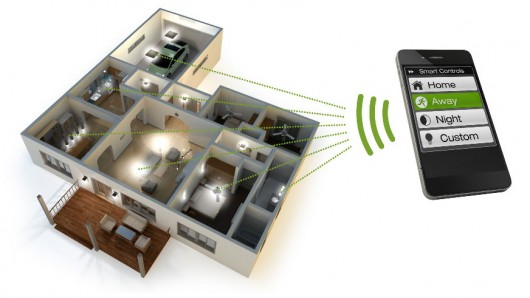
\includegraphics[width=0.48\textwidth]{fig/InternetOfThings}
\vspace{-10pt}
\caption{Internet of Things}
\vspace{-10pt}
\end{wrapfigure}
De komende jaren zal de omvang van het Internet exploderen omdat steeds meer van deze dagdagelijkse objecten ermee verbonden zullen worden. Het Internet zal evolueren naar een ‘Internet of Things’ en zal ons toelaten om op een eenvoudige manier en van op afstand informatie te verkrijgen over apparaten en hun omgeving (bv. de temperatuur, een deurslot, de status van de wasmachine) en ermee te interageren (bv. sluiten van de deur, aanschakelen van de verwarming). Tot voor kort was het besturen van apparaten in je huis vanop afstand met een smartphone, computer, etc slechts een theorie, maar de realisatie hiervan is nu dichter dan ooit.

\subsubsection{Is het internet klaar voor het IoT?}
Een grote remming op de ontwikkeling van een IoT is het beperkte adresbereik van Internet Protocol versie 4 (IPv4)\nomenclature{IPv4}{Internet Protocol versie 4}, maar met de invoering van Internet Protocol versie 6 (IPv6)\nomenclature{IPv6}{Internet Protocol versie 6} voor de deur, wordt het aantal mogelijke adressen aanzienlijk groter.
Alhoewel IPv6 blijkbaar voldoet aan de eisen voor het IoT zal de invoering van IPv6 op grote schaal nog even op zich laten wachten. Daarom zal het IoT voorlopig beperkt blijven tot testomgevingen en netwerken op kleinere schaal.\\
Een tweede probleem wordt gevormd door het verkeer dat zo'n sensornetwerk veroorzaakt. Huidig gebruikte protocollen zijn niet geoptimaliseerd voor verkeer van en naar een sensornetwerk. Het HyperText Transfer Protocol (HTTP)\nomenclature{HTTP}{HyperText Transfer Protocol} bijvoorbeeld, biedt een zeer betrouwbare vorm van communicatie, maar om die betrouwbaarheid te realiseren is een aanzienlijke hoeveelheid overhead nodig. Het is deze nood aan een lightweight protocol dat aan de oorzaak ligt van de recente ontwikkeling van het CoAP protocol. Het spitst zich toe op communicatie met minimale overhead. Als gevolg moet het CoAP protocol inboeten aan betrouwbaarheid. Het maakt immers gebruik van het minder betrouwbare User Datagram Protocol (UDP)\nomenclature{UDP}{User Datagram Protocol}. Daar waar HTTP juist betrouwbaarheid biedt, garandeert UDP niet dat alle pakketten effectief hun bestemming bereiken of dat die in volgorde aankomen.\\
De conclusie is dat het Internet in het geheel en onder zijn huidige vorm nog niet klaar is voor het IoT, maar dat niets in de weg staat van de ontwikkeling ervan in de zeer nabije toekomst.


\section{Doel}

Omwille van deze evolutie worden er meer en meer embedded devices ontwikkeld voor het IoT. Deze masterproef behandelt voornamelijk de integratie van die embedded devices in bestaande systemen. De focus ligt dan niet zozeer op de ontwikkeling van de embedded devices zelf, maar op het aanspreken en besturen van de embedded devices. Meer specifiek willen we een bijdrage leveren aan de realisatie van webservices voor het IoT. Het vertrekpunt hiervoor zullen de recente Constrained Application Protocol (CoAP)\nomenclature{CoAP}{Constrained Application Protocol}-ontwikkelingen zijn van de iMinds-onderzoeksgroep (C++ CoAP framework, HTTP-CoAP proxy, CoAP voor sensoren…). Als embedded device gebruiken we sensoren aangeboden door iMinds die bereikbaar zijn onder de vorm van een sensornetwerk.\\

Deze webservice bieden we aan onder de vorm van een Drupal-module waarbij een gebruiker een device rechtstreeks op locatie kan aanspreken door middel van native CoAP communicatie zonder dat er een proxy aan te pas komt. Dit is een groot verschil met recente implementaties waarbij er gebruik gemaakt wordt van een HTTP/CoAP proxy tussen de applicatie en het device. Concreet worden er twee modules ontwikkeld. Een CoAP library die al het berichtverkeer stuurt en afhandelt en een sensormodule waarin de gegevens afkomstig van de devices, verwerkt en weergegeven worden. De modules moeten zo ontwikkeld worden dat ze op een eenvoudige manier te gebruiken zijn, zodat geen kennis van de technische aspecten vereist is.\\

\section{Verloop masterproef}
Voor de eigenlijke ontwikkeling van de Drupal-module werden verscheidene boeken geraadpleegd, waarbij voor de implementatiedetails van het CoAP protocol, de CoAP drafts werden geraadpleegd.\\
In een eerste fase van deze masterproef zal de Drupal-module wel nog gebruik maken van een HTTP/CoAP proxy. Wanneer deze eerste fase geoptimaliseerd is, wordt de proxy uitgesloten en wordt er enkel nog gebruik gemaakt van het CoAP protocol.\\

Na een uitgebreide literatuurstudie van Drupal en PHP Hypertext Preprocessor (PHP, de gebruikte programmeertaal)\nomenclature{PHP}{PHP Hypertext Preprocessor} werd gepoogd een testmodule te maken. Het resultaat van deze eerste module bestond uit een webservice die dynamisch kon worden toegevoegd aan een Drupal website. Men kon deze webservice aanwenden om aan de hand van een Where On Earth ID (WOEID)\nomenclature{WOEID}{Where On Earth ID}, het weerbericht op te vragen van een plaats naar keuze.\\
De volgende stap bestond uit de ontwikkeling van een eerste versie van de uiteindelijk te ontwikkelen module. Deze bood de gebruiker de mogelijkheid om de waarde van \'{e}\'{e}n resource op te vragen. Bovendien kon de gebruiker met een checkbox aangeven of de waarde periodiek moest worden opgehaald. De opgehaalde waarden werden getoond in een tabel.\\
Na uitvoerig bestuderen van de CoAP drafts en het ontmantelen van CoAP berichten in Wireshark, werd ge\"{e}xperimenteerd met CoAP berichten. Al vlug bleek dat de ontwikkeling van een eigen CoAP library geschreven in PHP, de beste oplossing was. Aldus werd een aparte module ontwikkeld, een CoAP library die alle CoAP communicatie voor zich neemt. Deze module biedt de mogelijkheid tot opstellen, versturen en ontvangen van CoAP berichten.\\
Met de CoAP library voorhanden werd het nu mogelijk de sensormodule aan te passen zodat die enkel nog gebruik maakt van CoAP communicatie. Door deze laatste ontwikkeling werd ook de observe-methode van CoAP mogelijk, welke later toegelicht wordt.\\
Naast deze laatste ontwikkelingen die zich eerder toespitsen op de backend, werd ook vooruitgang geboekt aan de frontend. Een content-type werd ontwikkeld zodat een gebruiker gemakkelijk inhoud kan toevoegen aan zijn/haar website die voorzien wordt door onze module.\\
Omdat een gebruiker soms niet weet welke resources allemaal aangesloten zijn op een embedded device, wordt resource discovery voorzien. Dit houdt in dat de gebruiker enkel een IPv6 adres moet opgeven van een embedded device, waarna een lijst zal worden gegenereerd en getoond die alle resources bevat, aangesloten op dat embedded device.\\
Dit laatste concept wordt nog verder doorgedreven tot het concept van service discovery. Hierbij krijgt de gebruiker een overzicht van lijsten van resources van elk embedded device in een bepaald subnetwerk. Als alternatief gebruiken we een resource directory. Deze wordt ge\"{i}mplementeerd op een specifieke machiene waar alle embedded devices hun core op beschikbaar stellen. Een gebruiker kan deze directory aanroepen om toegang te krijgen tot alle well-known/cores.\\
Als laatste stap rest nog het samenvoegen van de frontend en backend. Als resultaat bekomt men dan een gebruiksvriendelijke module die de gebruiker in staat stelt sensoren te bekijken en te beheren zonder daarvoor enige kennis van onderliggende technologie\"{e}n nodig te hebben.


\section{Structuur scriptie}

In hoofdstuk twee gaan we dieper in op de concepten en mogelijkheden van CoAP. We bekijken het berichtformaat van CoAP en geven een vergelijking met HTTP. De voor- en nadelen komen eveneens aan bod. We bespreken de verschillende soorten communicatie en gaan ook dieper in op de concepten die met resource discovery te maken hebben. Deze concepten staan centraal in het automatiseren van sensorgegevens ophalen. %resource discovery moet mss in een appart hoofdstuk want dat is iets dat kan verwezenlijkt worden met CoAP maar dat is er geen deel van

Hoofdstuk drie handelt over Drupal. Ook hier geven we de voor-en nadelen en gaan we dieper in op de concepten: content-type, hook, module en blocks. We bekijken eveneens de werking van Drupal. Als laatste onderdeel van dit hoofdstuk bespreken we een voorbeeld van een Drupal module waarin jQuery gebruikt wordt. %kobe we plaatsen die weermodule dan bij dit hoofdstuk

In het vierde hoofdstuk bespreken we het concept en de implementatie 

In het vijfde hoofdstuk bespreken we de ontwikkelde CoAP library. %achtergrondprocessen, push vs pull, ... kan hierbij

In het zesde hoofdstuk bespreken we de sensormodule. %architectuur, geschiedenis van opgravingen, users, ... kan hierbij

Een mogelijk zevende hoofdstuk behandelt het ontwikkelen van een embedded device. Hiervoor werd als basis de Arduino UNO gekozen.











\chapter{Drupal} \label{Drupal}
\section{Wat is Drupal?}
\begin{wrapfigure}{r}{0.3\textwidth}
\vspace{-40pt}
%\hspace{-10pt}
\centering
\label{fig:drupalLogo}

\includegraphics[width=0.3\textwidth]{fig/drupalLogo}
\vspace{-30pt}
%\hspace{-10pt}
\centering
\caption{Drupal logo}
\centering
\vspace{-40pt}
\end{wrapfigure}
We kunnen Drupal het best beschrijven aan de hand van Figuur~\ref{fig:watIsDrupal}.
Drupal is een \textit{Content Management System} (CMS)\nomenclature{CMS}{Content Management System}, een \textit{framework} voor webapplicaties en een \textit{social publishing platform}. Maar Drupal is meer dan software alleen. Drupal staat voor een gemeenschap van ontwikkelaars en gebruikers met uiteenlopende doeleinden die elk hun eigen visie willen realiseren.~\cite{drupalDefGuide}

\subsubsection{Content Management System}
Drupal levert alle functies en mogelijkheden van een krachtig CMS. We denken meteen aan het kunnen inloggen en registreren van gebruikers, verschillende soorten gebruikers kunnen defini\"{e}ren, verschillende niveaus van permissies,... Ook denken we aan het cre\"{e}ren, aanpassen, beheren, weergeven, categoriseren en aggregeren van content. Drupal biedt bovendien de mogelijkheid om modulair extra functionaliteit toe te voegen naar eigen noden en wensen.

\subsubsection{Framework voor webapplicaties}
Drupal is zeer flexibel en krachtig waardoor er enorm veel verschillende soorten webapplicaties mee kunnen gebouwd worden. Dit is deels te danken aan de API's die Drupal aanbiedt. Deze worden bij elke versie van Drupal uitgebreid maar ze worden niet complexer om te gebruiken. % Drupal's veelzijdigheid wordt nogmaals bewezen met het feit dat het zowel als \textit{frontend} voor Java-gebaseerde applicaties kan optreden als voor \textit{backend} voor AJAX of Flash-driven \textit{frontend}s.

\subsubsection{Social publishing platform}
Dat Drupal een \textit{social publishing platform} is, houdt in dat content gemakkelijk te delen is via Drupal. Drupal biedt de mogelijkheid complexe data in een structuur te gieten die gemakkelijk uit te wisselen is. Op deze manier is het eenvoudig hetzelfde stuk content voor te stellen op verschillende websites.

\begin{figure}[h]
\centering
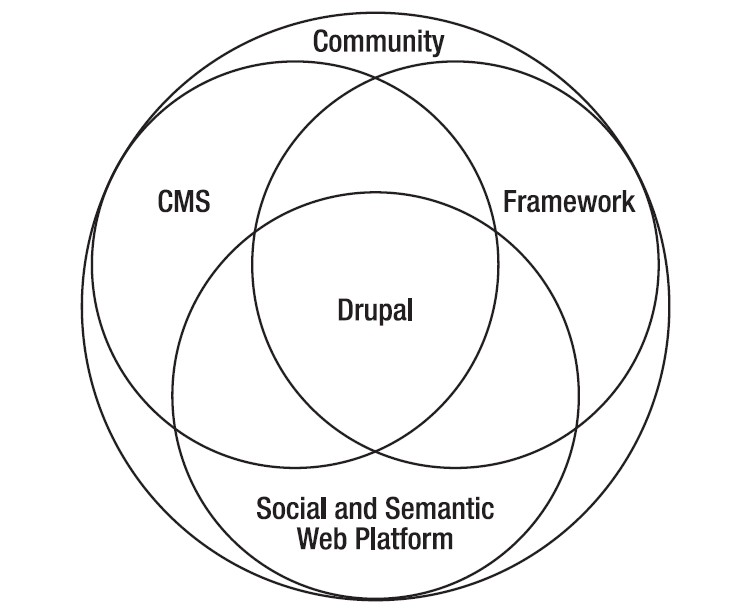
\includegraphics[width=0.4\textwidth]{fig/watIsDrupal}
\caption{Wat is Drupal?}
\vspace{-10pt}
\label{fig:watIsDrupal}
\end{figure}

We kunnen Drupal ook beschrijven als een gratis softwarepakket dat je de mogelijkheid biedt om jouw inhoud gebruiksvriendelijk te beheren en te publiceren. En dit op zo een manier dat je een eindeloze graad van personalisering hebt. Deze inhoud kan bestaan uit allerlei dingen, zoals: een blog, een video, een foto, een artikel, resultaten van een experiment,... Algemeen is dit dus een combinatie van tekst, beelden en audio die bezoekers van je website kunnen zien, lezen en/of horen. Bovendien is Drupal \textit{open source}.\\

Bij de implementatie van Drupal worden een aantal technologie\"{e}n gebruikt. De eerste is de \textit{HTML-embedded} \textit{scripting}taal PHP wat voor PHP: Hypertext Preprocessor staat. Het wordt gebruikt om dynamische webpagina's te cre\"{e}ren. PHP wordt \textit{server-side} uigevoerd, de code wordt op een webserver uitgevoerd. Dit in tegenstelling tot \textit{client-side}talen waar de code in een browser uitgevoerd wordt aan de clientzijde. De syntax van PHP bevat elementen van C, Java en Perl. Vanaf de huidige versie (PHP5) wordt object-ge\"{o}rienteerd programmeren ondersteund. Het is echter nog steeds mogelijk volledig proceduraal te werken.\\

Voor de \textit{frontend} wordt er een noemenswaardige hoeveelheid JavaScript in de vorm van jQuery gebruikt.\\

Als laatste wordt voor het opslaan van content en configuratiegegevens van Drupal een relationele databank gebruikt. Welke specifieke technologie als achterliggende databank gebruikt wordt kan zelf gekozen worden. Door in code gebruik te maken van de Database Abstraction Layer heeft deze keuze geen invloed op de Drupal code. Standaard wordt het gebruik van deze laag in combinatie met MySQL, SQLite of PostgreSQL ondersteund. Indien een andere technologie gekozen wordt, is er extra configuratie nodig. De Database Abstraction Layer wordt verder besproken in \ref{databaseAbstractionLayer}.\\

\noindent
Drupal in zijn huidige versie (7) kan op elk platform draaien onder volgende twee voorwaarden:
\begin{itemize}
\item Het platform bevat een webserver die PHP, en dus \textit{server-side} \textit{scripting} ondersteunt. Voorbeelden van deze webserver zijn:  Apache, IIS, Lighttpd en nginx.
\item Het platform ondersteunt een van volgende databanktechnologie\"{e}n: MySQL, SQLite of PostgreSQL.
\end{itemize}
Bij deze masterproef wordt er gebruik gemaakt van Apache en MySQL.

\subsection{Basiswebsite}
Wanneer je Drupal installeert beschik je meteen over een basiswebsite. Omdat je meteen al een bruikbare website hebt, is de drempel om Drupal te beginnen gebruiken dus laag. Deze website biedt meteen al een heleboel functionaliteit aan die geleverd wordt door de zogenaamde Drupal\textit{core}. %en een aantal out-of-the-boxfuncties.
\begin{figure}[h]
\begin{center}
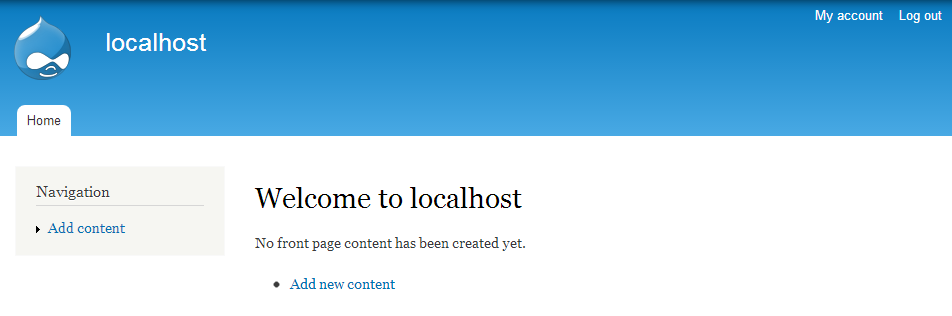
\includegraphics[keepaspectratio,width=1\textwidth]{fig/drupalBasiswebsite}
\vspace{-10pt}
\caption{Basiswebsite van Drupal met Bartik-theme}
\vspace{-30pt}
\end{center}
\end{figure}

\section{Waarom Drupal?}
We bekijken de principes waarop Drupal gebouwd is \cite{drupalMission}:
\begin{itemize}
\item Modulair en uitbreidbaar: Drupal kan uitgebreid worden met modules, waarbij je zelf ook modules kan ontwerpen indien er nog geen bestaat die aan jouw noden voldoet.
\item Kwaliteitsvolle codering: kwaliteitsvolle, elegante en goed gedocumenteerde code is een prioriteit.
\item \textit{Standard-based}: Drupal maakt gebruik van ingeburgerde standaarden zoals bijvoorbeeld XHTML en CSS.
\item \textit{Low-resource demanding}: om een goede prestatie te garanderen, maakt Drupal gebruik van low-profile codering (bijvoorbeeld minimaliseren van databasequeries).
\item \textit{Open source}: Drupal is gebouwd op, en kan gebruikt worden in, andere \textit{open source}projecten.
\item Gebruiksvriendelijk: Drupal moet gemakkelijk te gebruiken zijn. Zowel voor gebruikers, ontwikkelaars en administrators van een website.
\item Samenwerking: Drupal voorziet systemen om samenwerking te bevorderen, waaronder het versiebeheersysteem GIT.
\end{itemize}

\noindent
Een bijkomend voordeel van Drupal is zijn grote gemeenschap die ondertussen uit al meer dan 630000 actieve gebruikers en ontwerpers bestaat die zich dagelijks inspannen om Drupal steeds beter te maken. Dit aantal neemt elke dag toe. Veel van deze ontwikkelaars werken in hun vrije tijd aan het Drupal concept. Er zijn echter ook een aantal bedrijven die bijdragen leveren. Een van deze bedrijven is Acquia \cite{acquia}, een bedrijf gesticht door Dries Buytaert, de geestelijke vader van Drupal. Acquia biedt een aantal diensten aan voor zowel gebruikers en ontwikkelaars:
\begin{itemize}
\item Er werd gepoogd de drempel om Drupal te gebruiken te verlagen door onder andere de installatie te beperken tot het uitvoeren van een file. \item Begeleiding onder de vorm van video's, extra documentatie, allerlei tutorials en een helpdesk die 24/7 bereikbaar is via mail of telefoon.
\item Elastische resources om \textit{spikes} in netwerkverkeer op te vangen.
\item \textit{Maintenance} van jouw Drupal site.
\end{itemize}

\noindent
We bespreken nu enkele nadelen van Drupal:
\begin{itemize}
\item Aangezien Drupal gebruik maakt van een databank, heb je een databankserver nodig, al dan niet op dezelfde fysieke server als de webserver.
\item Bovendien wordt telkens een pagina wordt opgevraagd, (een stuk van) de \textit{bootstrap}code uitgevoerd, waarbij ook nog eens de databank veelvuldig wordt geraadpleegd. 
Dit maakt Drupal relatief traag.
\item Drupal is zeer gebruiksvriendelijk en ideaal voor de eindgebruikers, die gemakkelijk en interactief inhoud willen toevoegen en beheren. 
Beginnende Drupal ontwikkelaars zullen evenwel merken dat Drupal een erg steile leercurve heeft.
\item Ook ben je afhankelijk van de Drupal gemeenschap en dus de goodwill van de andere leden. Dit is in veel gevallen een voordeel, maar wanneer je een probleem hebt, ben je niet zeker of er wel een oplossing voor bestaat. Indien je gebruik maakt van software verkegen via Acquia heb je dit probleem niet.
\item Tenslotte kan iedereen een module maken. Dit heeft natuurlijk zijn voordelen maar wanneer je een module van iemand anders gebruikt, ben je nooit zeker of de module zal onderhouden worden naar de toekomst toe en of er al dan niet bugs in zitten. Nogmaals, bij gebruik van software verkregen via Acquia is dit minder van toepassing.
\end{itemize}

\section{Werking van Drupal}

Aan de hand van een voorbeeld \cite{drupalDefGuide} proberen we de lezer een idee te geven van de werking van Drupal. Bekijk Drupal als een digitale postzegelsorteerder. Nodes in Drupal zijn te vergelijken met de postzegels en het concept van contenttypes in Drupal is vergelijkbaar met de verschillende soorten postzegels (postzegels van \euro~0,67, \euro~1,34, ... ). Naast contenttypes, kan je \textit{taxonomy} gebruiken om een verdere onderverdeling te maken in de postzegels. De mate waarin en de criteria waarop je je onderverdeling maakt, kan je zelf kiezen (land, kleur, ...). Je kan zelf ook extra criteria opgeven, zoals 'grekegen-van-oma'. Je kan \textit{taxonomy} ook gebruiken om metadata toe te voegen aan content. Views is het mechanisme dat je postzegels sorteert en weergeeft in de vorm van pagina's en \textit{Blocks}. Van deze pagina's en \textit{Blocks} kan je zelf grootte, vorm, kleur en andere criteria opstellen zodat je deze helemaal kan personaliseren. %In paragraaf \ref{drupalBouwstenen} bespreken we de verschillende Drupal concepten in detail.\\

%Het achterliggende design pattern dat gebruikt wordt in Drupal is het Presenstation-Abstraction-Control (PAC) pattern. 

%Zie Figuur~\ref{fig:drupalGrafischeWeergave}.

%\begin{figure}[h]
%\centering
%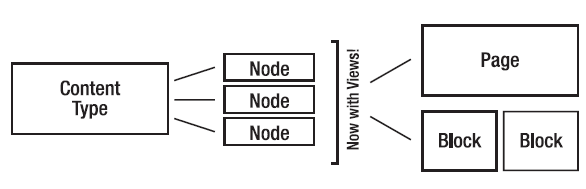
\includegraphics{fig/drupalGrafischeWeergave}
%\centering
%\vspace{-10pt}
%\caption{Grafische weergave van hoe Drupal content aanbiedt}
%\vspace{-10pt}
%\label{fig:drupalGrafischeWeergave}
%\end{figure}

\subsection{Drupal bouwstenen}\label{drupalBouwstenen}
We gaan dieper in op de begrippen die gebruikt werden in het postzegelsorteerdervoorbeeld en lichten enkele extra concepten toe die eveneens belangrijk zijn in Drupal.

\subsubsection{Contenttype}
Een contenttype bepaalt het soort content. Het bundelt soorten gegevens tot een logisch geheel. Wanneer content van een bepaald type wordt aangemaakt, worden de gegevens ingevuld door middel van \textit{Fields}. De toegevoegde content wordt een node genoemd. Ook biedt een contenttype de mogelijkheid om verschillende soorten content te onderscheiden van elkaar op basis van het type.
Drupal biedt gebruikers de mogelijkheid aan om hun eigen \textit{custom} contenttypes te maken. Hoe contenttypes aangemaakt en verwijderd worden wordt in paragraaf \ref{contenttypeManipulatie}.
%figuur van add contenttype

\subsubsection{Node}
Nodes zijn instanties van een contenttype. Een node kan maar aan \'{e}\'{e}n contenttype toebehoren.
Alle nodes hebben enkele eigenschappen gemeenschappelijk:
\begin{itemize}
\item Node id: zorgt voor een unieke identificatie.
\item Menu-instellingen: hier kan je een optionele menulink instellen zodanig dat je het menu op je website volledig kan personaliseren.
\item Mogelijkheden in verband met revisie: in de levensloop van de content kan je revisies maken zodat je terug kan keren naar een vorig moment indien er iets fout gaat met de content.
\item \textit{Uniform Resource Locator} (URL) \nomenclature{URL}{Uniform Resource Locator} pad instellingen: standaard is content beschikbaar via een URL van de vorm /node/node\_id. Maar via deze instellingen kan je een alias opgeven waarlangs de content ook (en dus gemakkelijker) beschikbaar is, dit principe heet in Drupal "\textit{Clean} URL's". De URL zal dan van de vorm /alias zijn.
\item Commentaarinstellingen: je kan zelf instellen of gebruikers commentaar kunnen achterlaten bij deze node.
\item Auteurinstellingen: hier stel je in of de creatietijd en auteur getoond moeten worden bij deze node.
\item Publicatieinstellingen: soms is het mogelijk dat je deze content nog niet beschikbaar wil stellen op de website, of je wil ze tijdelijk offline halen. Via deze instellingen is dit mogelijk.
\end{itemize}

\subsubsection{Fields}
Via \textit{Fields} kan je gegevens van een contenttype invullen. Standaard biedt Drupal een aantal velden aan om gegevens toe te voegen, zoals een tekstveld of een veld om een afbeelding mee te oploaden. Maar soms schieten deze velden tekort, bijvoorbeeld wanneer je een kalender met drie drop-downlists wil combineren om een datum en tijdstip bij elkaar te laten horen in een veld. Daarom heeft een gebruiker de mogelijkheid \textit{custom} velden te maken. Fields worden verder besproken in paragraaf~\ref{Fields}.

\subsubsection{View}
\textit{Views} worden gebruikt om content visueel voor te stellen op welke manier dan ook. Een \textit{view} is dan ook niet meer dan een visuele representatie van een verzameling content uit de databank.

\subsubsection{Block}
\textit{Blocks} zijn, zoals de naam impliceert, blokken die een verzameling van herbruikbare content bevatten. Ze geven het beeld van die content. \textit{Blocks} kunnen op gemakkelijke wijze toegevoegd worden aan je website waar jij dat wilt en hoe vaak je dat wilt. Het is bijvoorbeeld gemakkelijk om aan te geven dat je een bepaald \textit{Block} enkel op een bepaalde pagina wil laten verschijnen, en bovendien waar op de pagina je dat wilt. Merk echter wel op dat het hier niet echt content betreft, de inhoud van het \textit{Block} wordt aangemaakt bij opvraging en is dus geen blok beheerbare content. We zien een voorbeeld van een \textit{Block} in paragraaf~\ref{jQuery}.

\subsubsection{Theme}
\textit{Themes} zijn templates die bepalen hoe jouw website eruit ziet en aanvoelt voor de gebruiker. Net zoals modules zijn \textit{themes} modulair en zijn ze dus gemakkelijk te wisselen, ook \textit{themes} kunnen zelf ontwikkeld worden en zijn ter beschikking op de Drupal gemeenschap.

\subsubsection{Taxonomy}
Taxonomy geeft je de mogelijkheid om eigenschappen en categorie\"{e}n toe te voegen aan je content, zodat bijvoorbeeld een gebruiker content kan filteren uit een grote verzameling. Het biedt dus een manier om je content te organiseren. Een praktijkvoorbeeld is een receptensite, een gebruiker kan dan recepten filteren aan de hand van de eigenschappen van het gerecht (ingredi\"{e}nten, moeilijkheid, ...).

\subsubsection{Gebruikers, rollen en permissies}
%Gebruikers zijn personen die zich aangemeld hebben op jouw website, met uitzondering van de anonieme gebruikers.
Alle gebruikerfunctionaliteit zoals registreren, inloggen, enz... zit reeds in de Drupal \textit{core}. Rollen geven weer tot welk type een gebruiker hoort. Meerdere gebruikers kunnen dezelfde rol hebben, en een gebruiker kan meerdere rollen hebben. Met permissies kan je aangeven welke privileges een gebruiker met een bepaalde rol heeft en dus wat die gebruiker wel en niet mag doen. Deze permissies worden gekoppeld aan een rol zodat alle gebruikers die deze rol hebben automatisch de privileges hebben van deze rol. Drupal biedt standaard drie rollen aan: de Administratorrol, die alle privileges bevat; de geauthenticeerde gebruikerrol, die een aantal van de privileges van de Administratorrol bevat en de anonieme gebruikerrol, die een subset van de privileges van de geauthenticeerde gebruikerrol bevat. Anonieme gebruikers zijn gebruikers die zich niet aangemeld hebben op de website.

\subsubsection{Module}
Modules bieden de mogelijkheid om extra functionaliteit in te pluggen op een website. Modules zijn gratis te downloaden van de Drupal gemeenschap en omdat deze gemeenschap groot is, is de kans zeer groot dat er al een module gemaakt is voor jouw probleem. Indien dit niet het geval is, heb je nog altijd de mogelijkheid om zelf een module te ontwikkelen. Het gebruik van modules voorkomt ook dat functionaliteit die je niet nodig hebt, ook niet op jouw website komt. Je website is dus zeer configureerbaar naar eigen wensen (Zie figuur~\ref{fig:drupalOrganizeModules}).
\begin{figure}[h]
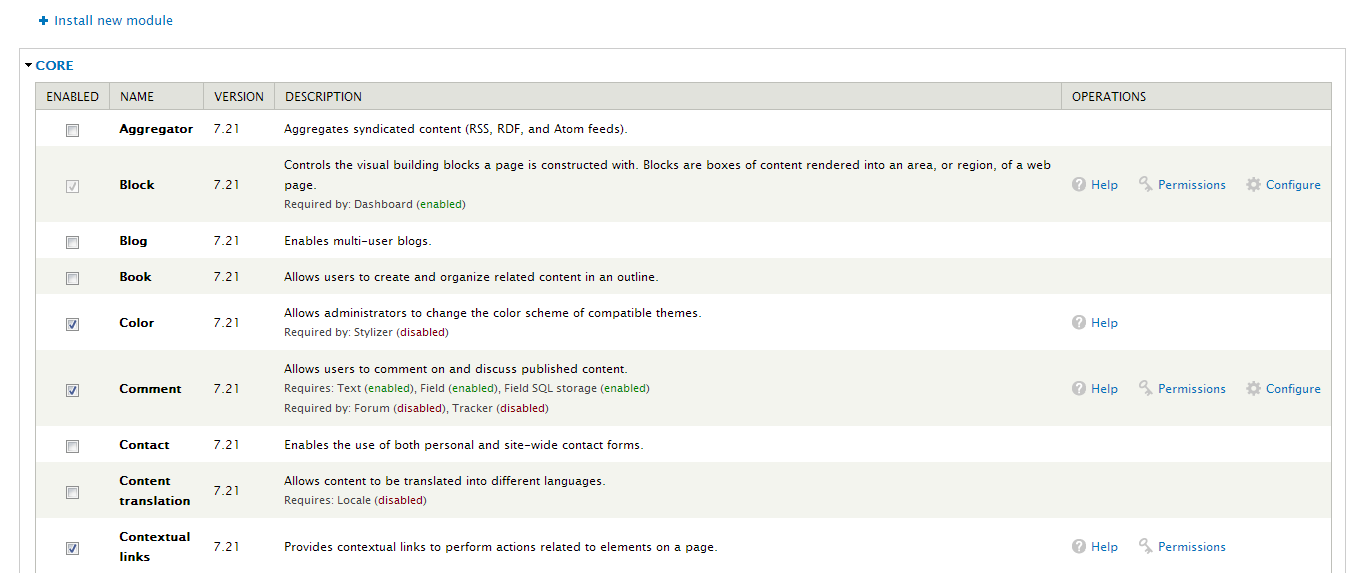
\includegraphics[width=1\textwidth]{fig/drupalOrganizeModules}
\caption{Organisatie van Drupal modules}
\label{fig:drupalOrganizeModules}
\end{figure}

\subsubsection{Drupal core}
De Drupal \textit{core} is wat je downloadt van de Drupal website. Het vormt de basis en een uitgebreide \textit{out-of-the-box} functionaliteit, het fungeert eigenlijk als de motor achter een Drupal website. De Drupal \textit{core} is zeer uitgebreid en complex, het vormt op zich al voldoende materiaal voor een scriptie, er verder op ingaan zou ons dus te ver leiden.

\subsubsection{Entities}
Een nieuw belangrijk concept in Drupal 7 is \textit{entities} \cite{entities}. Dit nieuwe concept in combinatie met de \textit{Entity API} heeft twee positieve effecten. Het eerste effect is dat gebruikers en commentaren dezelfde mogelijkheden krijgen als nodes. In vorige versies van Drupal was het niet mogelijk versies te cre\"{e}ren of velden toe te voegen aan gebruikers of commentaren. Andere voordelen zoals het gebruiken van \textit{views} in combinatie met gebruikers of commentaren was ook niet mogelijk. Het andere effect is het invoeren van object-ge\"{o}rienteerd programmeren van \textit{entities}. Vroeger was het nodig specifieke functies van de \textit{core} te gebruiken om content te bewerken. Een voorbeeld hiervan is node\_save() dat nodes opslaat. Deze functie was enkel toepasbaar op een node. Het alternatief bij de \textit{Entity API} is entity\_save(). Deze functie is niet gelimiteerd tot enkel content of enkel tot gebruikers.
Het is ook mogelijk nieuwe \textit{entities} te maken. %, we gaan hier dieper op in in hoofdstuk~\ref{uitbreidingen}.

\subsubsection{Hooks}
Hooks zijn functies die gedefinieerd zijn door de Drupal \textit{core}. Ze kunnen worden ge\"{i}mplementeerd door elke module. In de Drupal \textit{bootstrap} zal de Drupal \textit{core} dan op bepaalde tijdstippen de bijhorende \textit{hooks} oproepen van elke module die de \textit{hook} ge\"{i}mplementeerd heeft. Hiervoor wordt een zeer eenvoudig mechanisme gehanteerd. Een module kan zo'n \textit{hook} implementeren door de naam van de \textit{hook} te laten voorafgaan door de naam van de module die de \textit{hook} implementeert (zie codevoorbeeld~\ref{lst:drupalHookExample}).\\

\scriptsize
\lstset{language=PHP}
\begin{lstlisting}[label=lst:drupalHookExample,caption=Implementatie van hook\_node\_view door de module coap\_sensor]
function coap_sensor_node_view($node, $view_mode, $langcode) {
  if($node->type == 'coap_resource'){
    _coap_resource_add_js();
  }
  else if($node->type == 'coap_device'){
    $node->content['coap_device_form'] = drupal_get_form('coap_device_form', $node);
  }
  return $node;
}
\end{lstlisting}
\normalsize

\subsection{Database Abstraction Layer}\label{databaseAbstractionLayer}
Manipulatie van gegevens in de databank gebeurt via de \textit{Database Abstraction Layer} \cite{databaseAbstractionLayer}. Dit zorgt ervoor dat de implementatie van een module onafhankelijk is van de gebruikte soort databank. Concreet biedt deze laag een aantal functies aan voor het manipuleren van de databank. Wanneer een nieuw soort databank in gebruik genomen wordt, worden deze functies ge\"{i}mplementeerd voor deze nieuwe soort. We geven enkele voorbeelden van de meest gebruikte functies:
\lstset{language=PHP}
\begin{lstlisting}[label=db_select,caption=Voorbeeld gebruik van db\_select]
$result = db_select('coap_sensor_interested_user','resource')
	->fields('resource', array('nid'))
	->condition('uri', $uri, '=')
	->condition('uid', $user->uid, '=')
	->execute();
\end{lstlisting}
In voorbeeld \ref{db_select} wordt opgevraagd wat het nid is voor een specifieke uri en uid. Er wordt gebruik gemaakt van de Drupalvariabele \$user. Zoals je ziet moet er een naam opgegeven worden na de tabelnaam. Deze naam moet herhaalt worden als eerste element van de fieldstabel. Merk op dat dit alleen nodig is bij het gebruik van db\_select. Als tweede element van de fieldstabel geef je een tabel op met alle velden die je wil opvragen. Meerdere condities kunnen opgegeven worden, de volgorde is niet belangrijk. De opgevraagde gegevens kunnen gesorteerd worden door gebruik te maken van -\textgreater orderBy('nid', 'ASC').\\

De variabele \$result zal een \textit{SelectQuery}-object bevatten. Er zijn twee manieren om de opgehaalde gegevens uit objecten van deze klasse te halen. Wanneer je weet dat er maar een enkele rij opgehaald wordt, doe je best het volgende
\lstset{language=PHP}
\begin{lstlisting}
$record  = $result->fetchAssoc();
$nid = $record['nid'];
\end{lstlisting} 
Wanneer er meerdere rijen teruggegeven kunnen worden gebruik je beter
\lstset{language=PHP}
\begin{lstlisting}
$nids = array();
foreach($result as $record){
	$nids[] = $record->nid;
}
\end{lstlisting} 
om een tabel met al je gewenste resultaten in te bekomen. % In dit voorbeeld zal er echter maar \'{e}\'{e}n rij teruggegeven worden en is de eerste optie beter.
\lstset{language=PHP}
\begin{lstlisting}[label=db_insert,caption=Voorbeeld gebruik van db\_insert]
$id = db_insert('coap_sensor_interested_user')
	->fields(array(
		'uid' => $user->uid,
		'uri' => $resource_uri,
		'device' => 0,
		'nid' => $nid,
		'observe' => 0,
	))
	->execute();
\end{lstlisting}
In voorbeeld \ref{db_insert} wordt een entry toegevoegd aan de tabel coap\_sensor\_interested\_user. Kolommen die niet null mogen zijn en geen \textit{default}waarde hebben moeten opgegeven worden in de fieldstabel. Zoniet wordt er een exceptie opgegooid bij het oproepen van de execute-functie.

\lstset{language=PHP}
\begin{lstlisting}[label=db_update,caption=Voorbeeld gebruik van db\_update]
$num_updated = db_update('coap_sensor_interested_user')
	->fields(array(
		'new' => 0,
	))
	->condition('uid', $user->uid, '=')
	->condition('device',1,'=')
	->condition('nid', $nid, '=')
	->execute();
\end{lstlisting}
In voorbeeld \ref{db_update} wordt van alle rijen die overeenstemmen met de opgegeven condities de new-waarde op 0 gezet. % Bij dit voorbeeld zal er maar \'{e}\'{e}n rij geupdated worden.

\lstset{language=PHP}
\begin{lstlisting}[label=db_delete,caption=Voorbeeld gebruik van db\_delete]
db_delete('coap_sensor_interested_user')
	->condition('nid', $nid, '=')
	->execute();
\end{lstlisting}
In voorbeeld \ref{db_delete} worden alle rijen met als nid de waarde in \$nid verwijderd. % Opnieuw zal in dit voorbeeld maar \'{e}\'{e}n rij verwijderd worden.

\subsection{Laadcyclus van de pagina}
Wanneer een webbrowser een Drupal pagina opvraagt, wordt de Drupal URL van de pagina gebruikt. Deze heeft vaak volgende vorm: http://drupalvoorbeeld.org/node/15. De webserver vormt deze URL om naar de vorm: index.php?q=node/15 en geeft dan het pad node/15 door aan Drupal's index.php waarvan de code uitgevoerd wordt. Het uitvoeren van deze code resulteert in een reeks complexe stappen die als eindresultaat de gerenderde pagina hebben. Afhankelijk van het feit of de pagina al dan niet in de cache aanwezig is, verlopen deze stappen anders. Indien de pagina niet aanwezig is in de cache, wordt de volledige \textit{bootstrap} en de \textit{page callback} uitgevoerd. De \textit{bootstrap} bestaat steeds uit dezelfde reeks van acht verschillende fasen die we verder nader toelichten. Na de \textit{bootstrap} wordt de \textit{page callback} uitgevoerd die geassocieerd wordt met het pad meegegeven met index.php. Indien de pagina wel in de cache aanwezig is, wordt er enkel een aantal van de stappen van de \textit{bootstrap} uitgevoerd. De \textit{page callback} wordt in dit geval niet uitgevoerd. We bespreken elke stap van het proces apart, het hele proces wordt weergegeven in Figuur~\ref{fig:drupalPageRendering}.

\begin{figure}
\centering
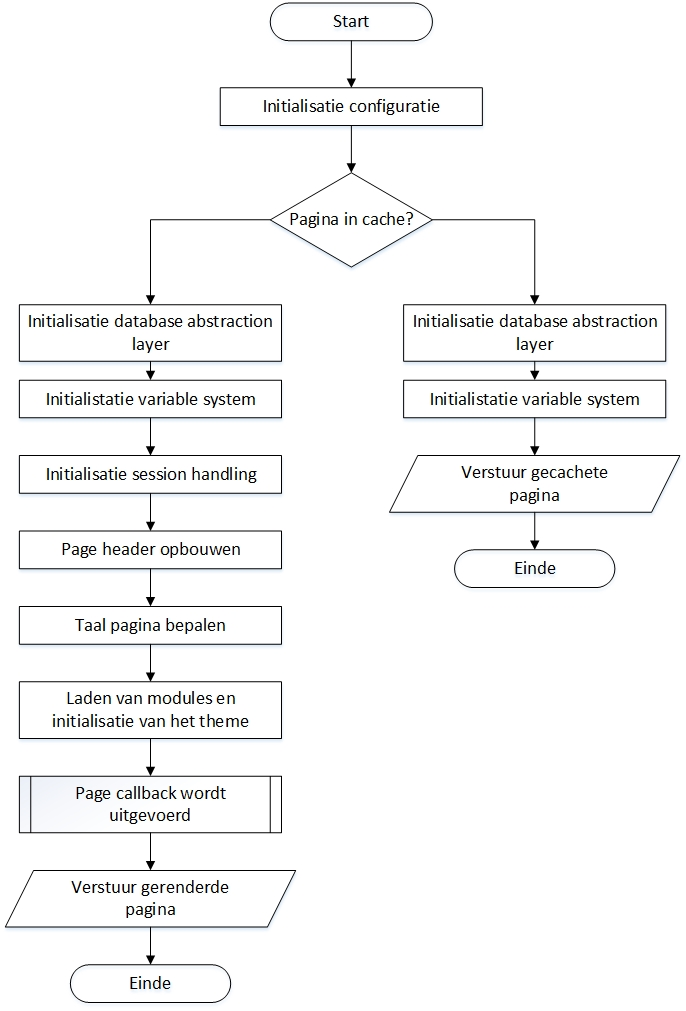
\includegraphics[width=1\textwidth]{fig/drupalPageRendering}
\caption{Laadcyclus van de pagina in Drupal}
\label{fig:drupalPageRendering}
\end{figure}

\subsubsection{Initialisatie van de configuratie}
Deze fase houdt onder andere in dat globale variabelen worden gezet, zoals de basis-URL van de website. Sommige waarden van deze variabelen worden rechtstreeks uit het configuratiebestand settings.php gehaald. Andere worden berekend aan hand van de omgeving waarin de server zich bevindt. In settings.php worden variabelen op opgegeven via de variabele \$conf. Deze variabele is een associatieve array die alle waarden op de variabelenaam mapt.

\subsubsection{Poging tot opvragen van een gecachte pagina}
Caching van pagina's treedt op indien page caching ge\"{e}nabled is. Bovendien gebeurt dit standaard enkel voor anonieme gebruikers. Er zijn echter modules beschikbaar om dit ook voor geauthenticeerde gebruikers te laten gebeuren. Het doel van caching is vermijden dat de volledige \textit{bootstrap} en \textit{page callback} moeten worden doorlopen om zo tijdswinst te cre\"{e}ren. De pagina  wordt enkel uit de cache gehaald als ze eerder is opgevraagd en nog steeds geldig is. De cache backend is pluggable en standaard gebruikt Drupal een databank cache implementatie. Deze cache backend heeft dus een databankconnectie nodig om de pagina op te halen. Daarom worden de volgende twee fasen (initialisatie van de Database Abstraction Layer en initialisatie van het Variable System) uitgevoerd voor de pagina effectief uit de cache kan gehaald worden. Dit wordt aangegeven door de stippellijnkaders in Figuur~\ref{fig:drupalPageRendering}. De cache backend en of caching al da niet ge\"{e}nabled is, wordt opgegeven in settings.php.

\subsubsection{Initialisatie van de Database Abstraction Layer}
Er zijn nog geen verbindingen met de databank nodig. Daarom worden enkel basisklassen en functies ge\"{i}nitialiseerd. Gebruik van de Database Abstraction Layer werd beproken in paragraaf~\ref{databaseAbstractionLayer}.

\subsubsection{Initialisatie van het Variable System}
In deze fase wordt gebruik gemaakt van de \textit{variable}tabel. Deze tabel heeft maar twee kolommen, \textit{name} en \textit{value} en beschrijft, zoals de naam zegt, variabelen. Alle name-valueparen worden uit de \textit{variable}tabel gehaald en toegevoegd aan de variabelen gedefin\"{i}eerd in settings.php. Variabelen die al gedefin\"{i}eerd zijn in settings.php hebben een hogere prioriteit dan degene die uit de \textit{variable}tabel gehaald worden. Het nut van deze variabelen is configuratie toevoegen aan de Drupal website. De reden dat een tabel gebruikt wordt om deze variabelen op te slaan is om de waarden persistent te maken. Wanneer de site offline gaat en terug online komt is de configuratie nog steeds beschikbaar. Drupal biedt ontwikkelaars een aantal functies aan om deze variabelen te manipuleren vanuit code:
\begin{itemize}
\item variable\_get(\$naam, \$default = NULL): De variabele wordt uit \$conf gehaald. Indien deze niet gedefin\"{i}eerd is wordt de waarde in \$default teruggegeven.
\item variable\_set(\$naam, \$value): De variabele wordt opgeslaan in \textit{variable}tabel en gezet in \$conf.
\item variable\_del(\$naam): De variabele wordt verwijderd uit de \textit{variable}tabel en uit \$conf.
\end{itemize}

\noindent
Naast alle variabelen worden de modules die nodig zijn in de \textit{bootstrap} geladen. Onder deze modules verstaan we modules die minstens een van volgende \textit{hooks} implementeerd: hook\_boot(), hook\_exit(), hook\_language\_init(), of hook\_watchdog(). Als laatste onderdeel van deze fase wordt het \textit{locking}mechanisme ge\"{i}nitialiseerd. Dit is nodig bij langdurige processen die parallel naast elkaar kunnen maar niet mogen uitgevoerd worden, we gaan hier niet verder op in.

\subsubsection{Initialisatie Session Handling}
In deze fase wordt aan elke geauthenticeerde gebruiker een sessie gekoppeld. Een anonieme gebruiker krijgt geen sessie toegewezen tenzij er iets in de sessie moet worden opgeslagen. In dat geval wordt een nieuw sessie ID gegenereerd en wordt een nieuw \textit{User}object gecre\"{e}rd met user id 0. Een andere manier dan de standaard databank gebasseerde manier om sessies af te handelen kan opgegeven worden in settings.php.

\subsubsection{Page Header opbouwen}
De eerste HTTP-\textit{headers} worden opgebouwd. Deze worden echter nog niet verstuurd, dit gebeurt pas op het einde van de cyclus. In deze fase vormt zich de eerste mogelijkheid voor modules om functionaliteit in te pluggen in de cyclus van het laden van de pagina. Dit gebeurt via hook\_boot(). Deze \textit{hook} wordt uitgevoerd voor het aanmaken van de HTTP-\textit{headers}.

\subsubsection{De taal van de pagina bepalen}
Als de website meerdere talen ondersteunt wordt in deze fase de gekozen taal van de gebruiker bepaald. Eens de gekozen taal vastgesteld is kunnen implemenaties van hook\_language\_init() gebruikt worden om taalafhankelijke variabelen in te stellen.

\subsubsection{Laden van modules en initialisatie van het theme}
Alle ge\"{e}nablede modules worden geladen en het \textit{theme} wordt ge\"{i}nitialiseerd. Modules hebben nog de kans nieuwe \textit{stream wrappers} toe te voegen en bestaande te wijzigen via de \textit{hooks} hook\_stream\_wrappers() en hook\_stream\_wrappers\_alter(). Met de hook hook\_url\_inbound\_alter() kunnen er wijzigingen uitgevoerd worden aan de URL die gebruikt werd om deze pagina op te roepen. Bij het instellen van het thema wordt gekeken wat het actieve thema is. Dit kan het default thema zijn, ingesteld met de UI, een thema gekozen door de gebruiker ingesteld met hook\_custom\_theme() of een thema specifiek gezet voor dit pad. Aan het einde van deze fase wordt hook\_init() opgeroepen. Dit wordt meestal gebruikt om globale parameters in te stellen die later in de request gebruikt worden.

\subsubsection{Uitvoeren van page callback}
Na het uitvoeren van de \textit{bootstrap} moet de pagina opgebouwd en gerenderd worden. Deze fase leggen we uit aan de hand van een voorbeeld.

\subsubsection{Voorbeeld}
We gaan uit van de specifieke URL http://drupalvoorbeeld.org/node/15 die we in het begin van deze paragraaf gebruikten. Op Figuur~\ref{fig:drupalPageCallback} zijn de hooks waarmee modules tussen beide kunnen komen worden aangegeven naast de respectievelijke fasen.\\

Drupal herkent het woord node in het pad en laadt de node met Node id = 15 via de functie node\_load(15). Gegevens van het node-object worden uit de databank gehaald en de hooks hook\_load(), hook\_entity\_load() en hook\_node\_load() worden opgeroepen zodat modules de kans krijgen het node-object te veranderen of extra acties te ondernemen. Tijdens het laden van de node worden velden geassocieerd met de node eveneens opgehaald. Dit gebeurt met field\_attach\_load(). Modules krijgen de kans de opgehaalde data van de velden te manipuleren met de hooks hook\_field\_storage\_pre\_load() en hook\_field\_attach\_load().\\

Nadat de node geladen is wordt hij doorgegeven aan de \textit{page callback}. Hier wordt hij omgevormd tot een \textit{renderable array}. Dit gebeurt met de functie node\_page\_view(). Het zet als paginatitel de titel van de node. Het voegt ook een canonical en short link toe aan de HTML head elemeents en de HTTP headers. In deze functie wordt de functie node\_show() gebruikt waarin de functie node\_view\_multiple() opgeroepen wordt die op zijn beurt node\_view() oproept waarin uiteindelijk de \textit{renderable array} gemaakt wordt. Via de hooks hook\_node\_view() en hook\_entity\_view() kunnen modules de \textit{renderable array} nog manipuleren. Met de hooks hook\_node\_view\_alter() en hook\_entity\_view\_alter() krijgen modules nog een kans om de array te manipuleren nadat andere modules al veranderingen doorgevoerd hebben.\\

Wanneer de \textit{renderable array} gemaakt is, en teruggegeven wordt door de \textit{page callback}, wordt hij doorgestuurd naar drupal\_deliver\_page() waarin drupal\_deliver\_html\_page() opgeroepen wordt die op zijn beurt de array rendert met drupal\_render(). Voor drupal\_render() effectief opgeroepen wordt, kunnen modules nog wijzigingen doorvoeren met de hook hook\_page\_build(). Modules kunnen nog een laatste keer tussenbeide komen met de hook hook\_page\_alter().

\begin{figure}
\centering
\hspace{55pt}
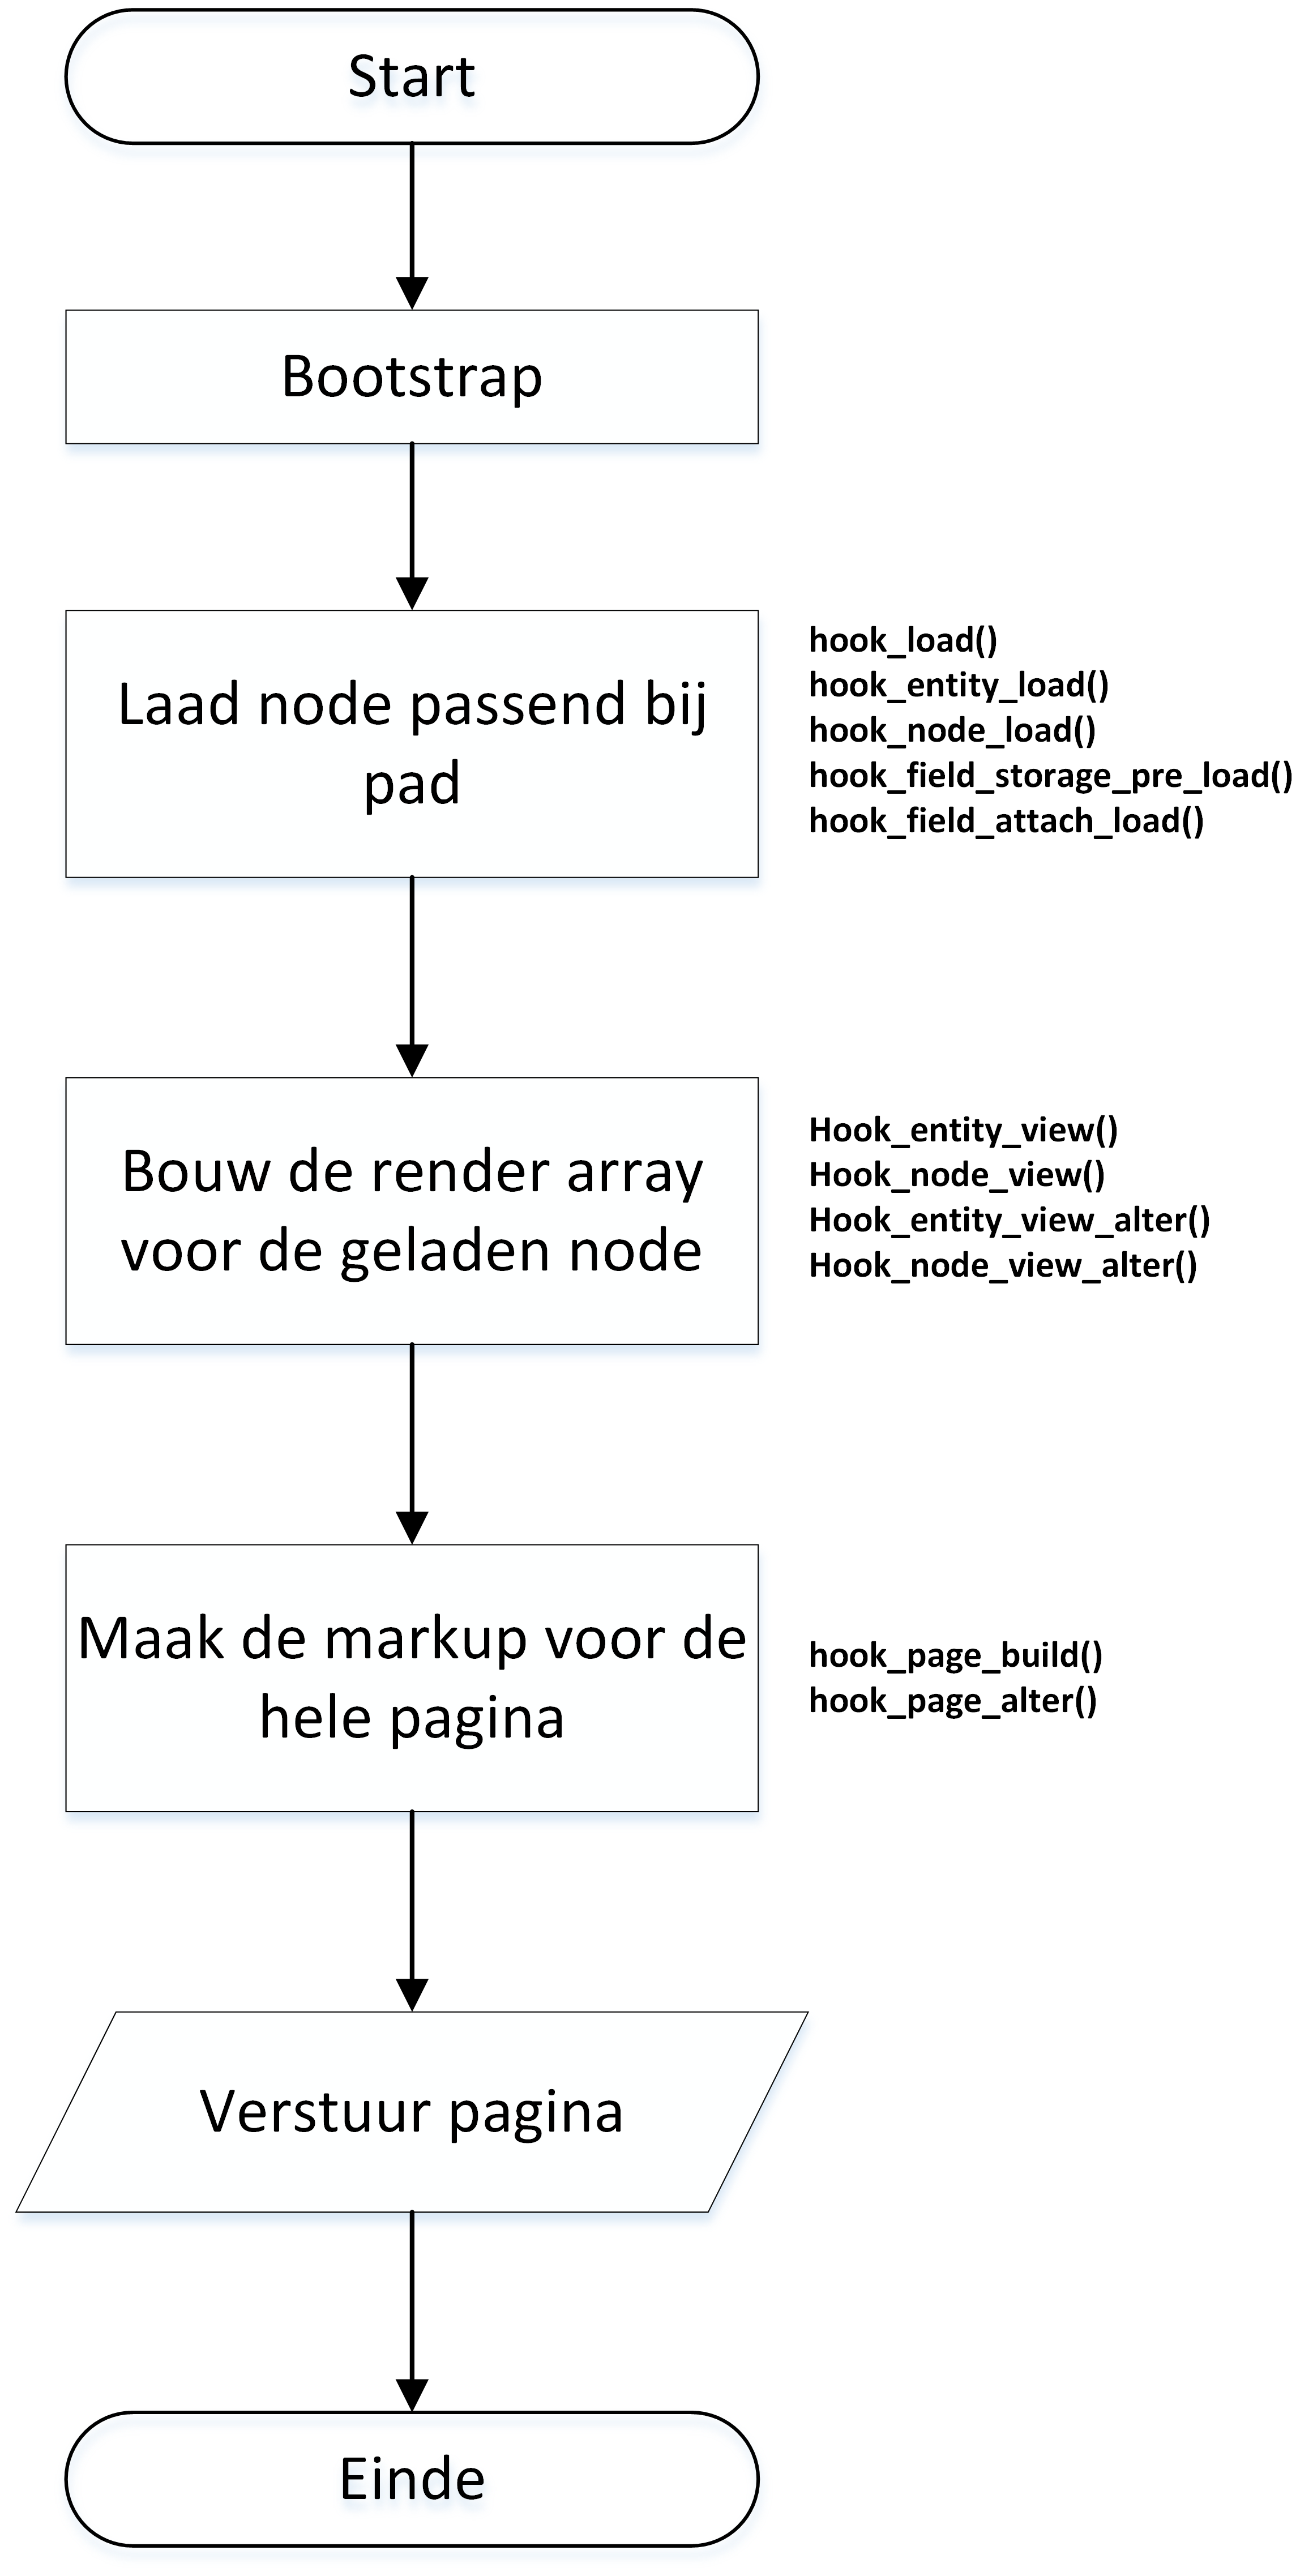
\includegraphics[width=0.65\textwidth]{fig/pageCallback}
\hspace{-50pt}
\caption{Voorbeeld van de laadcyclus van een pagina waar een node weergegeven wordt}
\label{fig:drupalPageCallback}
\end{figure}

\newpage

\subsection{Fields}\label{Fields}
Velden worden op een bepaalde manier behandeld in Drupal. We kunnen velden vergelijken met klassen. Wanneer een veld gebruikt wordt in een contenttype, wordt een instantie van deze klasse gemaakt. De gegevens van velden en hun instanties worden in verschillende tabellen in de databank opgeslaan.
\subsubsection{Fields in de databank}
De verschillende tabellen worden weergegeven in Figuur~\ref{fig:fieldtabellen}. We geven een korte beschrijving van deze tabellen:
\begin{itemize}
\item field\_config: Bevat algemene informatie over een veld. Een veld staat hier maar een keer in beschreven omdat deze informatie onafhankelijk is van de module waarin het gebruikt wordt.
\item field\_config\_instance: Bevat rijen per instantie van een veld. Een veld komt hier evenveel in voor als het aantal modules waarin het gebruikt wordt, rekening houdend met het aantal keer het voorkomt in een module. De informatie beschrijft dus de relatie tussen het veld en de modules waarin het voorkomt.
\item field\_data\_\textit{naam\_field}: Bevat de data bijhorende bij het veld. Data afkomstig van instanties die tot verschillende modules behoren worden in deze tabel opgeslaan. Er worden dus geen aparte datatabellen voorzien per instantie.
\item field\_revision\_\textit{naam\_field}: Bevat archiveringswaarden bijhorende bij verschillende \textit{revisions} van een instantie van een veld zodat teruggekeerd kan worden naar een vorige \textit{revision}.
\end{itemize}
\begin{figure}[h]
\centering
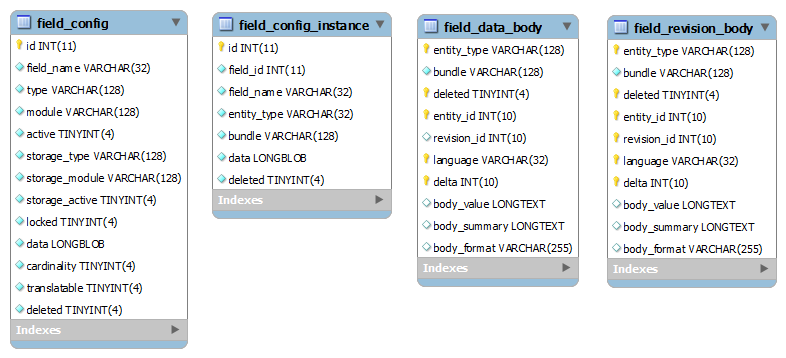
\includegraphics[width=1\textwidth]{fig/fieldtabellen}
\caption{Field tabellen}
\label{fig:fieldtabellen}
\end{figure}

\subsubsection{Aanmaken van Fields}
Velden kunnen aangemaakt worden met een GUI aangeboden door het Drupal systeem of ze kunnen aangemaakt worden vanuit code. Dit gebeurt dan best op het moment dat een module die ze nodig heeft ge\"{i}nstalleerd wordt, m.a.w. in de implementatie van hook\_install(). De velden worden aangemaakt met field\_create\_field(\$field) en de instanties worden aangemaakt met field\_create\_instance(\$instance). Hoe de argumenten voor deze functies opgebouwd zijn is beschikbaar in de Field CRUD API \cite{fieldCRUD}.

\subsubsection{Verwijderen van Fields}
Opnieuw kunnen velden verwijderd worden met een GUI aangeboden door het Drupal systeem of het kan vanuit code gebeuren. Via de GUI gebeurt dit impliciet door een contenttype te verwijderen. Achter de schermen wordt de functie node\_type\_delete(\$naam\_contenttype) opgeroepen en in deze functie wordt de functie field\_attach\_delete\_bundle(\$entity\_type, \$bundle) opgeroepen waar op zijn beurt de functie field\_delete\_instance(\$instance) oproept. Deze functies die achter de schermen opgeroepen worden wanneer de GUI gebruikt wordt, kunnen eveneens in code gebruikt worden.

\subsection{Modules}
Een extra woordje uitleg hoe een module wordt toegevoegd en verwijderd uit een Drupal systeem kan geen kwaad. We merken meteen op dat er naast de\"{i}nstalleren van een module ook \textit{disablen} mogelijk is. Dit kan als gevolg hebben dat een beginnende Drupal ontwikkelaar veronderstellingen maakt die niet volledig kloppen. We maken een opsomming van handige feiten in verband met \textit{enablen}, \textit{disablen} en de\"{i}nstalleren voor beginnende Drupal ontwikkelaars:
\begin{itemize}
\item Bij \textit{disablen} wordt hook\_disable() opgeroepen. Dit is analoog voor \textit{enablen}, installeren en de\"{i}nstalleren.
\item Een gebruiker moet een module altijd eerst \textit{disablen} voor te de\"{i}nstalleren.
\item Een gebruiker kan een module enkel expliciet \textit{enablen}, \textit{disablen} of de\"{i}nstalleren. Een module wordt ge\"{i}nstalleerd als ze voor de eerste keer enabled wordt of eerst gede\"{i}nstalleerd werd voor te \textit{re-enablen}. Installeren kan dus enkel impliciet.
\item Sommige \textit{hooks} worden maar opgeroepen bij installatie van de module, wat betekent dat wanneer je een wijziging van deze \textit{hooks} wil doorvoeren, je de module moet \textit{disablen}, de\"{i}nstalleren en \textit{re-enablen}. De\"{i}nstallatie mag niet worden overgeslagen omdat de module dan niet geherinstalleerd wordt. Dit is van toepassing bij volgende \textit{hooks}:
\begin{itemize}
\item hook\_node\_info()
\item hook\_schema()
\end{itemize}
\end{itemize}

\subsection{Aanmaken en verwijderen van contenttypes}\label{contenttypeManipulatie}
\subsubsection{Aanmaken van contenttypes}
Er zijn meerdere manieren om contenttypes aan te maken en te configureren.
\begin{itemize}
\item Via een GUI die standaard aangeboden wordt door de Drupal website.
\item De functie node\_type\_save() gebruiken om een nieuw type op te slaan. Deze methode kan je overal in code gebruiken.
\item Hook\_node\_info() implementeren waarin je de nieuwe contenttypes beschrijft. Deze hook wordt enkel opgeroepen bij installatie van een module.
\end{itemize}
\noindent
De eerste optie is enkel interessant voor Drupal gebruikers die zelf geen module wensen aan te maken of voor ontwikkelaars die het effect op de databank van het aanmaken van een contenttype willen bekijken. De twee laatste functies kunnen door ontwikkelaars gebruikt worden om contenttypes aan te maken in code.De laatse optie wordt echter algemeen als de betere optie gezien omdat het gebruik van \textit{hooks} de \textit{Drupal way} is.
De laatste twee opties zijn echter niet voldoende om een contenttype volledig te configureren. Een aantal specifieke variabelen moeten toegevoegd worden in de \textit{variable}tabel. De variabelen die wij toevoegen, hebben een invloed op de configuratie van de contenttypes die we toevoegen.

De variabelen worden gezet in de implemenatie van hook\_enable() door de module die het contenttype definieert. Deze variabelen moeten voor elk contenttype gezet worden en bevatten de naam van het contenttype waar ze een invloed op hebben. Een volledige lijst van mogelijke variabelen die een invloed hebben op het contenttype vind je online \cite{contentTypeVariables}. We sommen degene op die we gebruiken:
\begin{itemize}
\item comment\_\textit{naam\_contenttype}: Krijgt de waarde 0 om \textit{default} commentaren uit te schakelen.
\item node\_options\_\textit{naam\_contenttype}: Krijgt de waarde array('status') om \textit{default} '\textit{Promote to Front page}' uit te vinken.
\item node\_preview\_\textit{naam\_contenttype}: Krijgt de waarde 0 om de mogelijkheid tot een preview te \textit{disablen}.
\item node\_submitted\_\textit{naam\_contenttype}: Krijgt de waarde 1 om \textit{default} de auteur en de tijd waarop de content is toegevoegd te tonen bij de content zelf.
\end{itemize}

\noindent
Een laatste stap die nog doorgevoerd moet worden is het cre\"{e}ren van de velden die toegevoegd gaan worden aan de contenttypes, vervolgens worden er instanties van de velden aangemaakt om ze te linken aan de contenttypes. Dit gebeurt in hook\_install(). Er worden velden aangemaakt voor: de URI van devices, de URI van resource en een veld voor meerdere referenties naar content van het type coap\_resource. Velden werden besproken in paragraaf~\ref{Fields}.

\subsubsection{Verwijderen van contenttypes}
De contenttypes worden verwijderd in hook\_uninstall(). Voor een contenttype kan verwijderd worden moeten nog een aantal andere zaken verwijderd worden. We overlopen de verschillende stappen die voor elk te verwijderen contenttype moeten overlopen worden:
\begin{itemize}
\item Alle content van het contenttype wordt verwijderd door middel van de functie\\ node\_delete\_multiple(\$nids). De variabele \$nid bevat een array met alle nids van de content die verwijderd wordt.
\item Alle variabelen die toegevoegd werden in de \textit{variable}tabel worden verwijderd door gebruik te maken van variable\_del(\$naam);
\item De comment-entiteit die geassocieerd is met dit contenttype wordt gemarkeerd om te verwijderen. Hiervoor wordt de functie field\_delete\_instance() gebruikt.
\item Het contenttype wordt verwijderd met node\_type\_delete(\$naam\_contenttype). In deze functie worden de instanties van de velden geassocieerd met dit contenttype ook verwijderd door gebruik te maken van de functie field\_attach\_delete\_bundle(\$entity\_type, \$bundle). We merken op dat de commentaren apart verwijderd werden.
\item De databankcache van node types wordt geupdated met node\_types\_rebuild(). Dit is nodig omdat Drupal vaak in caches kijkt en verouderde informatie kan gebruiken.
\item Drupal zal bij het verwijderen van velden de kolomwaarde deleted op 1 zetten. Om de velden effectief uit de databank te verwijderen wordt de functie field\_purge\_batch() gebruikt.
\end{itemize}

\section{JQuery in Drupal} \label{jQuery}

\begin{wrapfigure}{r}{0.25\textwidth}
\vspace{-40pt}
\hspace{-10pt}
\centering
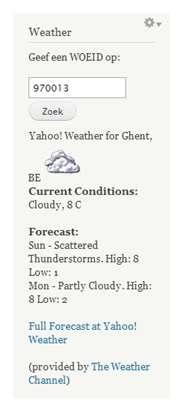
\includegraphics[width=0.3\textwidth]{fig/weermodule}
\vspace{-30pt}
\hspace{-10pt}
\centering
\caption{Weermodule}
\label{fig:weermodule}
%\centering
\vspace{-70pt}
\end{wrapfigure}

In deze paragraaf bekijken we hoe een module (weather\_info) gemaakt werd die het weerbericht ophaalt voor een regio naar keuze, aangegeven door een WOEID. In eerste instantie werd gewerkt met een formulier, maar in een latere fase werd overgestapt op jQuery, wat de gebruikerservaring bevordert.

\subsection{Met een HyperText Markup Language (HTML)-formulier} \nomenclature{HTML}{HyperText Markup Language}

In eerste instantie bevatte de module een formulier bestaande uit een tekstveld als invoer voor de WOEID en een knop om het formulier in te dienen.
Wanneer de gebruiker op de knop klikt, gebeuren volgende stappen:

\begin{itemize}
	\item het formulier wordt ingediend
	\item de pagina wordt opnieuw geladen
	\item de \textit{bootstrap}code roept hook\_form\_submit() op door weather\_location\_form\_submit() op te roepen (weather\_location is de naam van het formulier):
	\begin{itemize}
		\item het ingegeven WOEID wordt opgeslagen op serverniveau met de Drupal functie variable\_set()
	\end{itemize}
	\item de \textit{bootstrap}code roept hook\_block\_view op van de weermodule door weather\_info\_block\_view() op te roepen:
	\begin{itemize}
		\item het ingegeven WOEID wordt opgehaald met behulp van de Drupal functie variable\_get()
		\item er wordt een HTTP-\textit{request} uitgevoerd naar de \textit{Yahoo Weather API} met de PHP-functie file\_get\_contents(), dat een URL als parameter verwacht
		\item het ontvangen xml-bestand wordt in een object gestopt met de PHP-functie SimplexmlElement(), waarna het weerbericht gemakkelijk uit het XML-bestand kan gehaald worden
		\item Het weerbericht wordt toegevoegd aan de inhoud van het \textit{Block}
	\end{itemize}
	\item De pagina wordt in de browser weergegeven met het weerbericht in het \textit{Block}
\end{itemize}

\subsection{Met AJAX in jQuery}

Een pagina zal pas getoond worden wanneer de \textit{bootstrap} afgelopen is en aangezien de code in de \textit{hooks} die worden uitgevoerd onderdeel is van de \textit{bootstrap}, zal de pagina pas getoond worden wanneer de \textit{hooks} afgelopen zijn. Dit heeft als gevolg dat de gebruiker van de website langer moet wachten op de pagina omdat eerst nog een HTTP-\textit{request} moet gebeuren om het weerbericht op te halen. Het spreekt voor zich dat dit een zeer nadelig effect is dat moet vermeden worden.\\
Als alternatief hebben we gekozen om een jQuery-event te koppelen aan de submit-knop die het formulier indient. jQuery is namelijk geschreven in JavaScript en JavaScript is een \textit{client-side \textit{scripting} language}, wat inhoudt dat deze code wordt uitgevoerd op de machine van de gebruiker en dit nadat de pagina geladen is.\\
Wanneer de gebruiker op de knop klikt, wordt een \textit{Asynchronous JavaScript and XML}(AJAX)-\textit{call}\nomenclature{AJAX}{Asynchronous JavaScript and XML} uitgevoerd.
Zoals de naam suggereert, is dit een asynchrone aanroep, wanneer het antwoord aankomt, wordt automatisch een opgegeven functie opgeroepen waarin de data kan verwerkt worden. Als gevolg heeft de gebruiker dus geen enkele hinder van het internetverkeer dat noodzakelijk is om het weerbericht op te halen.


\subsection{Problemen}

JQuery laat geen \textit{cross-domain} AJAX \textit{calls} toe wegens veiligheidsoverwegingen. De \textit{Weather Service API} bevindt zich namelijk op een ander domein. Een oplossing hiervoor is een \textit{proxy}script in PHP gebruiken.
De AJAX-\textit{call} gebeurt dan naar het \textit{proxy}script dat zich op de server en dus hetzelfde domein bevindt. Het \textit{proxy}script vraagt daar effectief de data op en geeft de uitvoer terug.
De browser wordt dus eigenlijk om de tuin geleid. \cite{crossDomainProblem}

\chapter{CoAP} \label{CoAP}

\section{Wat is CoAP?}

CoAP is een web transfer protocol speciaal ontwikkeld voor netwerkcomponenten die beperkt zijn in zowel geheugen als energieverbruik, als in machine-to-machine (M2M)\nomenclature{M2M}{Machine-to-machine}communicatie. Met M2M-communciatie bedoelen we communciatie tussen machines waar geen menselijke tussenkomst nodig is. Zoals de berichten die routers naar mekaar sturen om hun routingtabel te synchroniseren. Naast het minimaliseren van overhead concentreert CoAP zich ook op het automatiseren van taken. Het mechanisme van resource discovery (Zie paragraaf \ref{resourceDiscovery}) is hier een voorbeeld van. Met het verminderen van energieverbruik in het achterhoofd biedt CoAP naast synchrone ook asynchrone communicatie aan. Het biedt ook nieuwe soorten berichten aan zoals non-confirmable, piggy-backed, etc. Deze worden toegelicht in paragraaf \ref{betrouwbaarheid}\\


Het interactiemodel van CoAP is vergelijkbaar met het client/server model van HTTP. Hoewel, bij een CoAP implementatie voor M2M interacties kan een device bij de ene berichtuitwisseling client zijn, en bij de andere server. Een CoAP request is equivalent aan een HTTP request en wordt ook gestuurd van de client naar de server om een actie aan te vragen op een resource die zich op die server bevindt. De actie wordt bepaald door een method code (GET, PUT, POST of DELETE) en de resource wordt aangeduid met een Uniform Resource Identifier (URI).\nomenclature{URI}{Uniform Resource Identifier} De server antwoordt met een response die onder andere een response code bevat.\\

Verschillend met HTTP, gebeurt de berichtenuitwisseling asynchroon over een datagram-ge\"{o}ri\"{e}nteerd transport. Dit houdt in dat berichten mogelijks verloren gaan of in een andere volgorde kunnen aankomen dan dat ze verzonden zijn. Toch voorziet CoAP enige vorm van betrouwbaarheid met een soort bericht dat kan worden bevestigd door een acknowledgement (zie paragraaf \ref{betrouwbaarheid}). Wanneer zo'n bericht niet wordt bevestigd, wordt het bericht meermaals opnieuw gestuurd volgens het exponential back-off mechanisme (Zie paragraaf \ref{exponentialBackoff}).

CoAP definieert vier soorten berichten: Confirmable, Non-confirmable, Acknowledgement en Reset. Door gebruik te maken van method codes en response codes transporteren sommige van deze berichten requests of responses. In paragraaf \ref{communicatieMogelijkheden} gaan we hier dieper op in.\\

\begin{wrapfigure}{r}{0.5\textwidth}
\vspace{-10pt}
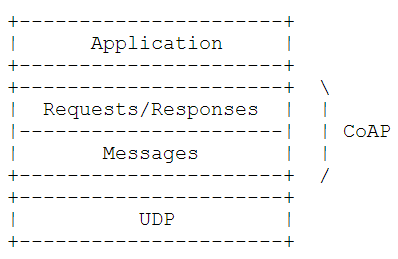
\includegraphics[width=0.5\textwidth]{fig/CoAPLaag}
\vspace{-30pt}
\caption{CoAP lagen (CoAP 14 draft)}
\vspace{-5pt}
\label{fig:CoAPLaag}
\end{wrapfigure}
We kunnen CoAP ook in het Open Systems Interconnection (OSI) -model \nomenclature{OSI}{Open Systems Interconnection} met 7 lagen plaatsen. Logisch gezien hebben we een CoAP berichtenlaag die het UDP gedeelte en de asynchroniteit van de berichten afhandelt en een request/response laag die gebruik maakt van method en response codes (zie Figuur~\ref{fig:CoAPLaag}). Nochtans bestaat CoAP in werkelijkheid slechts uit \'{e}\'{e}n laag waarbij berichtenuitwisseling en het request/response-mechanisme enkel en alleen door manipulatie van de header verwezenlijkt wordt.

\subsection{Berichtformaat}

\begin{wrapfigure}{r}{0.7\textwidth}
\vspace{-20pt}
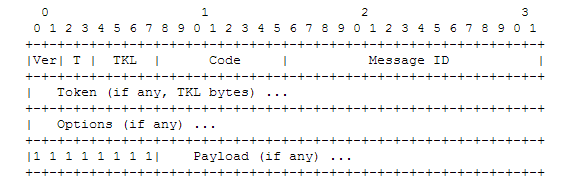
\includegraphics[width=0.7\textwidth]{fig/CoAPMessageFormat}
\vspace{-30pt}
\caption{Berichtformaat (CoAP 14 draft)}
\vspace{-10pt}
\label{fig:CoAPMessageFormat}
\end{wrapfigure}
Om een minimale overhead te realiseren worden de berichten zeer compact gehouden. We geven een kort overzicht van de onderdelen van het berichtformaat (zie Figuur~\ref{fig:CoAPMessageFormat}) en bespreken dan de belangrijke delen apart in subparagrafen. De eerste vier bytes stellen de header voor. Bemerk dus dat de header gerealiseerd wordt met slechts 4 bytes. Het veld na de header is optioneel en bevat een token waarvan de lengte aangegeven is in de header. Vervolgens zitten er nul of meer opties in het bericht.
Het laatste onderdeel van een bericht is de payload. Indien er een payload aanwezig is in het bericht, wordt die altijd voorafgegaan door een vaste byte, de payload marker (0xFF). Deze geeft het einde van de opties en het begin van de payload aan. Indien er geen payload is mag deze marker niet aanwezig zijn.

We merken hier op dat een token, opties en een payload optioneel zijn. Dit zorgt ervoor dat sommige berichten beperkt blijven tot de header van 4 bytes, wat zeer weinig is.

\subsubsection{Header}

Deze vier bytes worden opgedeeld in drie delen:
\begin{itemize}
\item Versiegetal (Ver): een 2-bit unsigned integer die de CoAP versie aangeeft. 
\item Type-aanduiding (T): een 2-bit unsigned integer die het berichttype aangeeft. De mogelijkheden zijn: Confirmable (CON) \nomenclature{CON}{Confirmable CoAP message} (0), Non-confirmable (NON)) \nomenclature{NON}{Non-Confirmable CoAP message} (1), Acknowledgement (ACK) \nomenclature{ACK}{Acknowledgement CoAP message} (2) of Reset (RST) \nomenclature{RST}{Reset CoAP message} (3).
\item Tokenlengte (TKL)\nomenclature{TKL}{ToKen Length}: een 4-bit unsigned integer die de variabele tokenlengte aangeeft.
\item Code: 8-bit unsigned integer die aangeeft of het bericht een request of een response overbrengt, of leeg is.
\item Message ID: een 16-bit unsigned integer die gebruikt wordt om duplicatie van berichten op te merken. Het wordt ook gebruikt om berichten van het type ACK/RST te linken aan berichten van het type CON/NON.
\end{itemize}

\subsubsection{Token}

Een token wordt gebruikt om een response te linken aan een request. De lengte wordt bepaald door de TKL en is nul tot acht bytes lang. Elk bericht heeft een token, dit kan lengte nul hebben. Wanneer een token nodig is, moet dat worden gegenereerd door de client. Indien de server wil dat zijn response geaccepteerd wordt, moet hij dit token zonder meer overnemen in zijn response.

\newpage

\subsubsection{Opties}

%\begin{wrapfigure}{r}{0.6\textwidth}
%\vspace{-20pt}
%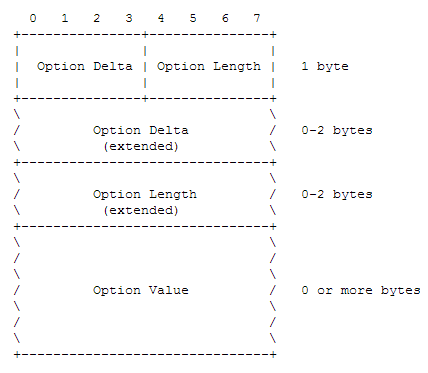
\includegraphics[width=0.6\textwidth]{fig/CoAPOpties}
%\vspace{-40pt}
%\caption{CoAP optie (CoAP 14 draft)}
%\vspace{-10pt}
%\label{fig:CoAPOpties}
%\end{wrapfigure}
Opties worden opgesteld door middel van de Type-Length-Value (TLV)\nomenclature{TLV}{Type Length Value} notatie (zie Figuur~\ref{fig:CoAPOpties}). Er wordt een mechanisme toegepast om opties in een pakket te stoppen, dat ervoor zorgt dat het pakket compact blijft en dus bijdraagt tot een minimale overhead.\\

Elke optie heeft een uniek nummer, maar wanneer meerdere opties in \'{e}\'{e}n pakket worden gestopt, worden de opties niet door dat nummer aangeduid, maar door de Option Delta. De Option Delta is het verschil tussen het nummer van een optie en dat van de vorige optie.
Concreet, stel dat men na een optie met nummer 6 een optie met nummer 11 wil plaatsen, dan wordt deze laatste aangeduid met Option Delta gelijk aan 5 (11 - 6). Dit alles samen maakt dat een minimale (lege, maar daarom niet nutteloze) optie slechts 1 byte in beslag neemt. Dit heeft als gevolg dat opties na elkaar moeten worden geplaatst met oplopende Option Numbers.\\

Indien de Option Delta 13 of meer is, schiet dit systeem tekort. Daarom zijn er speciale waarden ingevoerd die het gebruik van extended een extended Option Delta aangeven. Indien de Option Delta groter is dan 12, maar kleiner is dan 269, wordt als Option Delta waarde 13 gebruikt. Er wordt dan een extra byte voor de Option Value gezet dat opgevuld wordt met de echte Option Delta - 13. Indien de Option delta meer is dan 268, wordt als Option Delta de waarde 14 gebruikt. Deze waarde geeft aan dat er twee extra bytes gebruikt worden. Deze bytes worden opgevuld met de echte Option Delta - 269. De waarde 15 mag niet als Option Delta gebruikt worden want deze geeft het begin van de payload aan. Voor Option Length zijn de regels analoog.


\begin{figure}[h]
\centering
%\vspace{10pt}
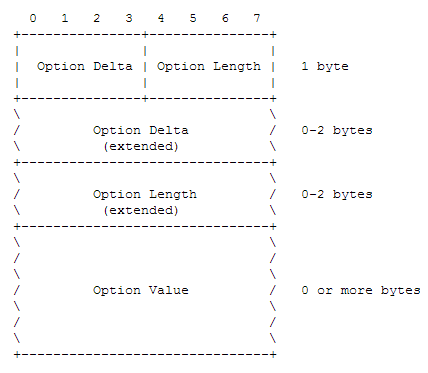
\includegraphics[width=0.6\textwidth]{fig/CoAPOpties}
\vspace{-10pt}
\caption{CoAP optie (CoAP draft 16)}
\label{fig:CoAPOpties}
\end{figure}

\newpage

\subsubsection{Verschil met HTTP}

Als we dit kort vergelijken met het berichtformaat van HTTP (zie Figuur~\ref{fig:HTTPMessageFormat}) zien we dat er aanzienlijke verschillen zijn. Bij HTTP zijn request en response niet helemaal gelijk. We kijken eerst naar de HTTP request.

Deze is opgedeeld in drie delen. Een requestlijn die op zijn beurt opgedeeld is in drie delen, gescheiden door een spatie. Het eerste deel is de methodenaam (GET, POST, HEAD, PUT of DELETE voor HTTP 1.1). Het tweede deel is de URL van de gevraagde resource en het laatste deel is het versienummer. Vervolgens zijn er een aantal headerlijnen die bijkomende opties voorstellen. De entity body wordt gebruikt door de POST methode om gegevens door te sturen en wordt gescheiden van de headerlijnen door een lege lijn. Bijkomend wordt elke lijn (ook de lege) afgesloten met een carriage return (CR)\nomenclature{CR}{Carriage Return} en een line feed (LF\nomenclature{LF}{Line Feed}).

De HTTP response is analoog aan de request met als verschillen dat de eerste lijn opgebouwd is uit het versienummer, de statuscode die aangeeft wat het resultaat van de request inhoudt en een korte beschrijving van de status code.\\
Het is dus duidelijk dat een HTTP bericht aanzienlijk groter zal zijn dan een CoAP bericht.

\begin{figure}[h]
\vspace{10pt}
\centering
\subcaptionbox{Request}
{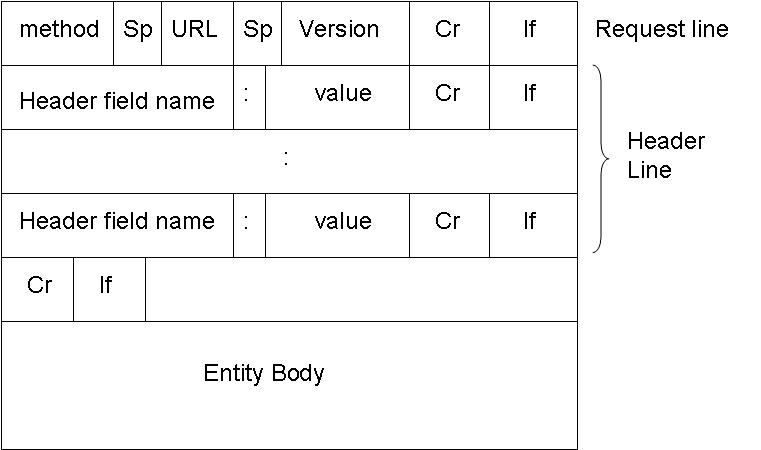
\includegraphics[width=0.45\textwidth]{fig/HTTPRequestMessageFormat}}
\subcaptionbox{Response}
{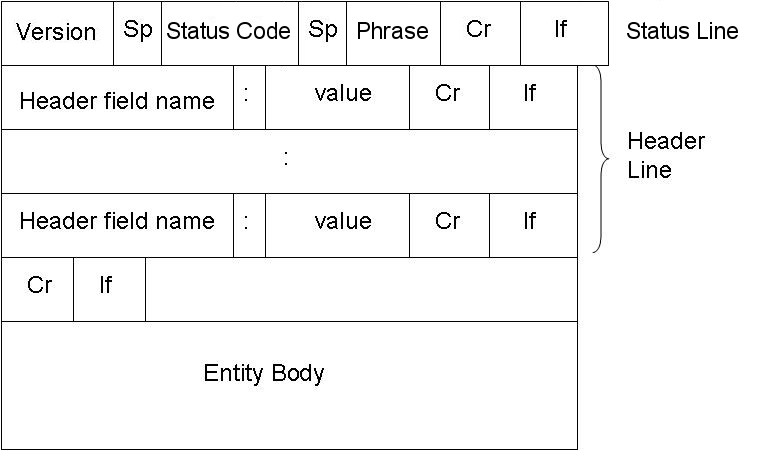
\includegraphics[width=0.45\textwidth]{fig/HTTPResponseMessageFormat}}
\caption{HTTP Message Format}\label{fig:HTTPMessageFormat}
\end{figure}

\newpage

\section{Communicatiemogelijkheden} \label{communicatieMogelijkheden}

In deze paragraaf bespreken we de communicatiemogelijkheden van CoAP. We bekijken de variabele betrouwbaarheid van CoAP berichten en gaan na hoe het request/response model bij CoAP werkt aan de hand van voorbeelden. Als laatste lichten we het principe van blockwise transfer even toe.

\subsection{Betrouwbaarheid} \label{betrouwbaarheid}

HTTP realiseert een betrouwbare en robuuste vorm van communicatie. Het is gebaseerd op het Transmission Control Protocol (TCP), dit protocol zet een verbinding op aan de hand van stream sockets. Het zorgt ervoor dat pakketten gegarandeerd aankomen bij de bestemming en dit in volgorde van verzending. Maar deze betrouwbaarheid komt met een prijs, namelijk extra netwerkbelasting voor het opzetten en beheren van die verbinding. In tegenstelling tot HTTP dat gebouwd is op TCP, is CoAP gebaseerd op berichtenuitwisseling over UDP. Wanneer men met dit protocol werkt, is er echter geen garantie dat pakketten aankomen en wanneer dat wel het geval is, kan de volgorde van aankomst gewijzigd zijn ten opzichte van verzending. Daarom moet men bij CoAP zelf de betrouwbaarheid verzorgen indien nodig.

\subsubsection{Confirmable berichten}

Wanneer we de betrouwbaarheid van de berichtenuitwisseling willen opdrijven, merken we de berichten als CON. Een CON-bericht moet door de server worden beantwoord met een ACK-bericht (zie Figuur~\ref{fig:berichtuitwisseling}), dit ACK-bericht moet hetzelfde message ID bevatten als het CON-bericht waarop geantwoord wordt. Wanneer CON-berichten niet worden beantwoord met een ACK-bericht v\'{o}\'{o}r een bepaalde timeout, wordt het bericht opnieuw verzonden. Bij het opnieuw verzenden wordt een exponential back-off mechanisme toegepast. Eerst wordt een timeout bepaald tussen een ACK\_TIMEOUT en ACK\_TIMEOUT x ACK\_RANDOM\_FACTOR, wanneer die timeout verstrijkt wordt het CON-bericht opnieuw verzonden en de timeout verdubbeld. Wanneer de server niet in staat is het CON-bericht te verwerken, wat betekent dat die zelfs geen geldige error response kan geven, antwoordt die met een RST-bericht in plaats van met een ACK-bericht.

\subsubsection{Non-confirmable berichten}

Soms heeft een bericht geen betrouwbaar transport nodig. Een voorbeeld hiervan is een stroom van sensordata waarbij elke meting verstuurd wordt met een NON-bericht. Dit soort berichten wordt niet bevestigd met een ACK bericht, maar de berichten hebben wel nog steeds een message id om duplicatie van berichten te detecteren (zie Figuur~\ref{fig:berichtuitwisseling}). Wanneer een ontvanger niet in staat is het bericht te verwerken, opnieuw bedoelen we daarmee dat het geen geldige error response kan geven, zendt die een RST-bericht naar de zender.

\begin{figure}[h]
\vspace{10pt}
\centering
\subcaptionbox{Confirmable}
{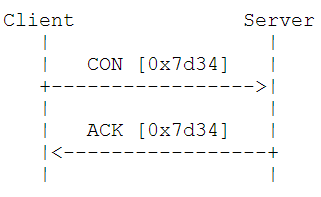
\includegraphics[width=0.3\textwidth]{fig/CoAPConfirmable}}
\hspace{30pt}
\subcaptionbox{Non-confirmable}
{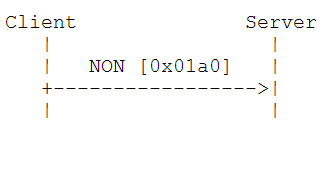
\includegraphics[width=0.3\textwidth]{fig/CoAPNonConfirmable}}
\caption{Berichtuitwisseling (CoAP 14 draft)}
\label{fig:berichtuitwisseling}
\end{figure}

\subsection{Request/response model}

\subsubsection{Piggy-backed response}

Wanneer een request met een CON bericht verstuurd wordt, is het mogelijk dat het antwoord meteen beschikbaar is bij de server. Indien dit het geval is, wordt het antwoord op de request meteen meegestuurd met het ACK bericht. Dit wordt een piggy-backed response genoemd. In Figuur~\ref{fig:CoAPPiggyBacked} worden twee voorbeelden van GET requests met piggy-backed responses getoond. De ene is succesvol, de andere geeft een error response terug.
\begin{figure}[h]
\vspace{10pt}
\centering
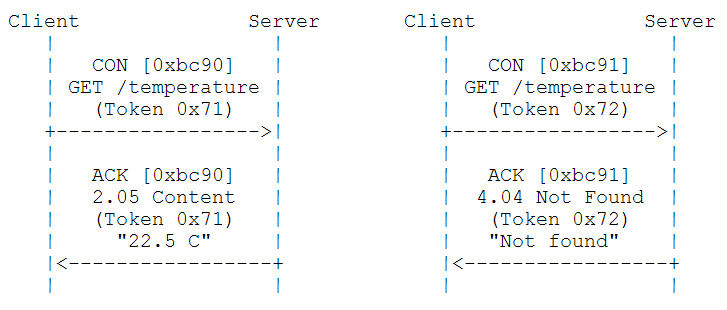
\includegraphics[width=0.7\textwidth]{fig/CoAPPiggyBacked}
%\vspace{-10pt}
\caption{Twee GET requests met piggy-backed responses (CoAP 14 draft)}
\label{fig:CoAPPiggyBacked}
\vspace{-20pt}
\end{figure}

\newpage

\subsubsection{Separate response} \label{separate}

\begin{wrapfigure}{r}{0.3\textwidth}
\vspace{-40pt}
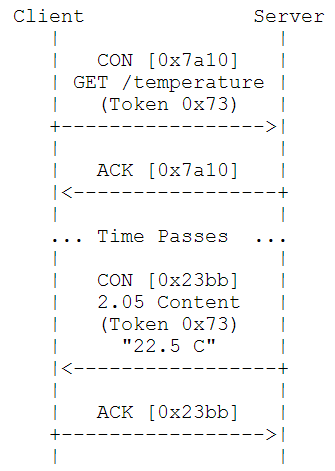
\includegraphics[width=0.3\textwidth]{fig/CoAPSeperateResponse}
\vspace{-30pt}
\caption{GET request met seperate response (CoAP 14 draft)}
\label{fig:SeparateResponse}
\vspace{-100pt}
\end{wrapfigure}
Wanneer de server niet onmiddellijk kan antwoorden op de request van de client, antwoordt die met een leeg ACK bericht zodat de client niet zou beginnen heruitzenden als gevolg van het exponential back-off mechanisme. Wanneer de response klaar is, stuurt de server dit antwoord in een nieuw CON bericht dat op zijn beurt beantwoord moet worden door de client. Dit soort van berichtenuitwisseling heet separate response (zie Figuur~\ref{fig:SeparateResponse}).
\\
\\
\\

\subsection{Blocks} \label{blocks}
CoAP werkt goed als de berichten geen of kleine payloads bezitten. Dit mag je veronderstellen als je werkt met temperatuursensors of lichtschakelaars. Maar soms is het nodig dat applicaties berichten sturen met grotere payloads, zoals bij resource discovery dat we in \ref{resourceDiscovery} bespreken of bij resources die nu eenmaal veel gegevens als antwoord op een request hebben.\\

Bij HTTP doet TCP al het werk om de pakketten te fragmenteren en ervoor te zorgen dat de deelpakketten in de juiste volgorde verwerkt worden. Dit is niet mogelijk bij CoAP aangezien UDP als transportprotocol gebruikt. Bij UDP zijn er ook verschillende niveau's van mogelijke fragmentatie, maar gebruik van deze niveau's moet vermeden worden om de fragmentatie af te handelen op applicatieniveau. Op deze manier worden meerdere blokken informatie van een enkele resource representation uitgewisseld via meerdere request-response paren. Belangrijk op te merken hierbij is dat elk request-response paar afzonderlijk af te handelen is door client en server. Dit heeft als gevolg dat er geen connectie opgezet moet worden en dat de server geen geheugen moet vrijmaken om bij te houden welk blok hij moet versturen. Welke de niveau's zijn en waarom er voor de Block Options gekozen is wordt uitvoerig besproken in de draft 'Blockwise transfers in CoAP' \cite{blockwiseTransfer}.

\subsubsection{Block Options}
Om grote payloads op een goede manier te ondersteunen worden twee Block Options ingevoerd. Optie 23 heeft als naam Block2 en geeft informatie over de request payload. Optie 27 heeft als naam Block1 en geeft informatie over de response payload. Beide opties  geven een blockwise transfer aan en kunnen zowel in requests als responses voorkomen. Ze ondersteunen blokgroottes die een macht van twee zijn, beginnend bij 16 t.e.m. 1024 bytes.

\subsubsection{Structuur}
Bij beide opties hebben de optiewaarden dezelfde structuur. De lengte van de waarde is variabel en kan 1, 2 of 3 bytes lang zijn zoals te zien in figuur~\ref{fig:blockOption}.
\begin{figure}[h]
\centering
\includegraphics[width=0.6\textwidth]{fig/blockOption}
\caption{Blokoptiewaarde - bytes en bits worden aangegeven bovenaan de figuur}
\label{fig:blockOption}
\end{figure}

\noindent
Wat we nog uit figuur~\ref{fig:blockOption} halen is dat het telkens drie elementen bevat:
\begin{enumerate}
\item NUM (Block Number): het relatief nummer van het blok binnen een sequentie van blokken.
\item M (More Flag): is dit het laatste blok in een reeks?
\item SZX (Size Exponent): geeft de grootte van het blok.
\end{enumerate}

\noindent
De blokgrootte is ge\"{e}ncodeerd gebruik makend van een drie-bit unsigned integer. 0 komt overeen met $ 2^{4} $ en 6 komt overeen met  $ 2^{10} $. Concreet wordt de grootte van het blok gegeven door  $ 2^{ SZX + 4} $. 7 mag niet gebruikt worden als waarde omdat deze gereserveerd is.

\section{Extra Features}

\subsection{Observe} \label{observe}

Wanneer een resource observable is of anders gezegd, de observe functionaliteit ondersteunt, kan die resource op eigen initiatief data sturen naar eventueel ge\"{i}nteresseerde clients. Een client kan zijn interesse uiten door een CON bericht te sturen naar de server dat een lege Observe Option (optie 6) bevat. Wanneer de client dan een ACK bericht terug krijgt met een observe option, weet die dat de server de client heeft toegevoegd aan de lijst van observers. Een client kan aangeven aan de server dat die niet meer ge\"{i}nteresseerd is door een RST bericht te sturen naar de server. De server verwijdert de client dan uit de lijst van ge\"{i}nteresseerden.

\subsection{Resource discovery} \label{resourceDiscovery}
Resource discovery zorgt ervoor dat lokale client en servers elkaar kunnen vinden en met elkaar kunnen interageren zonder menselijk tussenkomst.

\subsubsection{Principe}
\noindent
Resources kunnen maar aangesloten zijn op een device. Dit device maakt een fictieve resource aan met als naam de well-known/core. Deze fictieve resource bevat een opsomming van alle resources verbonden met dit device en een aantal gegevens over deze resources onder de vorm van attributen. Sommige well-known/core's bevatten ook verwijzingen naar resources op andere devices. Gebruikers kunnen een GET-request sturen om de well-known/core op te halen en hebben dan deze informatie tot hun beschikking. De well-known/core bevat echter veel informatie die niet in een enkel request-response paar uitgewisseld kan worden. Daarom wordt er gebruik gemaakt van blocks welke uitgelegd worden in \ref{blocks}. De manier waarop deze informatie doorgegeven wordt, is door gebruik te maken van het CoRE Link Format \cite{coapDiscovery}.

\subsubsection{CoRE Link Format}
Er worden geen resources opgeslaan in de well-known/core maar links naar deze resources. Als formaat van de links moet het CoRE Link Format gebruikt worden. Een resource wordt uniek ge\"{i}dentificeerd met een uri die tussen kleiner-dan (\textless) en een groter-dan (\textgreater) teken staat. Na de uri worden alle attributen opgesomd gescheiden door een puntkomma (;). De attributen zelf hebben de vorm van een name-value paar. Sommige attributen kunnen meerdere waarden hebben, deze waarden worden dan gescheiden door een spatie. Tot slot worden verschillende links gescheiden met een komma (,).\\

\noindent
Als voorbeeld geven we het antwoord op een GET-request van een well-known/core:\\
\textless/temp\textgreater;rt="temperature-c";if="sensor",\\
\textless/light\textgreater;rt="light-lux";if="sensor"\\
We zien dat het device met deze core twee resources aanbiedt. De eerste resource wordt ge\"{i}dentificeerd met de uri /temp, de andere met /light. Beide resources hebben twee attributen maar er zijn meer attributen mogelijk. We sommen de meest voorkomende attributen op:
\begin{itemize}
\item obs (Observable): Geef aan of de resouce observable is, indien deze optie ontbreekt wordt aangenomen dat de resource niet observable is.
\item rt (Resource Type): Geeft het type van de resource. De waarden zijn afhankelijk van de gebruikte applicatie. Ze hebben als nut dat binnen een applicatie, resources van hetzelfde type herkent kunnen worden. Dan kan via query filtering, alle resources van een type opgehaald worden.
\item ct (Content Type): Bevat een opsomming van de content formats die ondersteund worden door deze resource. 
\item if (Interface Description): Bevat een beschrijving van welke methoden deze resource ondersteunt.
\item sz (Maximum Size Estimate): Geeft aan hoe groot het maximum aantal gegevens ongeveer is als antwoord op een GET-request.
\item title: Bevat een omschrijving van deze resource.
\item anchor: 
\item rel: 
\end{itemize}
De lijst met alle attributen vind je in de CoRE Link Format draft \cite{coapDiscovery}.

\subsubsection{Core ophalen}
Om een well-known/core op te halen, moet je twee maal de Uri-Path Option (optie 11) toevoegen aan een GET-request die gericht is naar het IP-adres van het device waar de core zich op bevindt. De eerste keer met als value 'well-known' en de tweede keer gebruik je als value 'core'.\\

\noindent
We bespreken de eerste berichtenparen bij een resource discovery door de hexadecimale waarde te bekijken. Verschillende onderdelen scheiden we met een streep.\\

\noindent
De client stuurt een eerste discovery-request:\\
40 01 78 a5 \textbar~bb 2e 77 65 6c 6c 2d 6b 6e 6f 77 6e \textbar~04 63 6f 72 65\\
Het eerste deel bevat dezelfde elementen als elke GET-request. Het tweede deel bevat de eerste optie. De eerste twee bytes bevatten bb. Dit komt overeen met optie 11 met lengte 11. De 11 volgende byte-paren zijn de hexadecimale waarden van de karakters 'well-known'. Het laatste deel bevat ook een optie. Deze keer zijn de twee eerste bytes 04. De Option Delta is 0, dus hebben we opnieuw optie 11. De lengte is deze keer 4. De volgende byte-paren komen overeen met 'core'.\\

\noindent
Het antwoord van de server:\\
60 45 78 a5 \textbar~c1 28 \textbar~b1 0c \textbar~52 06 92 \textbar~ff ...\\
Het eerste deel is analoog aan andere responseberichten. We merken wel op dat de Message ID dezelfde is als de Message ID in de request van de client. De eerste twee bytes van het tweede deel zijn c1. Wat optie 12 (Content-Format) met lengte 1 impliceert. De waarde van deze optie is 28. Omgezet naar decimaal is dit 40, wat application/link-format aangeeft. Het volgende deel begint met b1. Dit komt overeen met optie 23 (Block2) met lengte 1. De hexadecimale waarde is 0c wat overeenkomt met 12 of binair 00001100. Als we dit herschikken zien we de elementen die in \ref{fig:blockOption} te zien zijn: 0000 1 110. We zien dat dit het nulde block is van een reeks van blocks met grootte 6 bytes. De 4-de laatste byte geeft aan dat er nog pakketten komen. Het voorlaatste deel begint met 52 wat optie 28 aanduidt met lengte 2. Het laatste deel begint met de payload marker waarop de payload volgt.\\

\noindent
De client stuurt een nieuwe request om het volgende pakket aan te vragen:\\
40 01 78 a6 \textbar~bb 2e 77 65 6c 6c 2d 6b 6e 6f 77 6e \textbar~04 63 6f 72 65 \textbar~c1 16\\
De eerste drie delen zijn analoog aan de eerste request. Het laatste deel dat erbij is gekomen geeft het volgende block aan dat verstuurd moet worden door de server. De eerste twee bytes zijn c1. Option Delta is 12 dus de optie is 11 + 12 = 23 (Block2). De lengte is 1 byte-paar. 16 binair is 0001 0 110. Het eerste block in de reeks van blocks met lengte 6 bytes wordt opgevraagd.\\

\noindent
De server zal met het aangevraagde block antwoorden. Dit proces blijft zich herhalen tot de server een response stuurt waar de M-bit op 0 staat.

\subsubsection{Query Filtering}
Het is mogelijk een specifieke discovery uit te voeren indien er enkel informatie over één resource moet gekend zijn of enkel de resources waarbij een bepaald attribuut een specifieke waarde heeft. Dit heeft als voordeel dat het netwerk niet overbodig belast moet worden als dat niet nodig is. De query-filter wordt voorgesteld door een name-value paar. Deze wordt toegevoegd door de Uri-Query Option (optie 15) te gebruiken.


\chapter{CoAP library module} \label{coaplibrary}

In hoofdstuk \ref{CoAP} bekeken we hoe het CoAP in mekaar zit en wat er allemaal mogelijk is. In dit hoofdstuk bekijken we hoe een eigen CoAP-\textit{library} in PHP werd ontwikkeld als Drupalmodule. De module stelt een Drupalgebruiker in staat CoAP-berichten op te stellen, te versturen en te ontvangen. Let wel, deze module heeft niet als doel om visueel iets voor te stellen op een website. Ze biedt enkel functionaliteit en is bijvoorbeeld te gebruiken in een andere module die dan uitgewisselde gegevens kan omvormen tot een visuele representatie. Dit laatste is wat wij doen in de uiteindelijk te ontwerpen module welke wordt toegelicht in hoofdstuk \ref{sensormodule}.

\section{Doel}

Wanneer we trachtten CoAP-berichten op te stellen, te versturen en ontvangen in onze module, werd al snel het nut duidelijk van een aparte module die zou fungeren als CoAP-\textit{library}. Er ontstaat namelijk erg veel duplicatie van code, bovendien wordt de code onoverzichtelijk en slordig. Nog een zeer nadelig gevolg is dat de code niet hergebruikt kan worden in andere modules. Men zou al de code moeten doorspitten om net dat stuk te vinden waar CoAP gesproken wordt. Bovendien is het niet zeker dat die code zal voldoen aan de waarschijnlijk andere eisen van de nieuwe gebruiker. Wanneer de code niet fungeert in de nieuwe situatie, zal er veel tijd gespendeerd moeten worden aan debuggen en zal de frustratie oplopen bij de gebruiker. Kortom, het is duidelijk dat dit een zeer slechte praktijk is die ten alle kosten moet vermeden worden, het druist in tegen enkele van de belangrijkste programmeerprincipes.\\

\newpage
Met het nut bewezen bekijken we even wat een gebruiker van deze \textit{library} kan verwachten. Ze moet de gebruiker in staat stellen dynamisch berichten op te stellen, volledig naar eigen wens. Dit wil zeggen dat de verzameling operaties om een bericht op te stellen, alle mogelijke berichten moet kunnen genereren. Dit heeft als gevolg dat elke elementaire operatie moet kunnen worden uitgevoerd op een bericht. Opstellen van bijvoorbeeld een bepaald bericht aan de hand van slechts \'{e}\'{e}n functie is niet prioritair en dus bijkomstig. Het is uiterst belangrijk bij het ontwerp van deze \textit{library} dat de gebruiker zich niet meer hoeft te bekommeren om technische details zoals hexadecimale code die nodig is in een bericht. Alle technische details zitten verborgen in de CoAP-\textit{library}module. We besluiten dat de \textit{library} een gebruiker in staat moet stellen dynamisch en gebruiksvriendelijk berichten op te stellen, en dit met een minimum aan code.

\subsection{Essenti\"{e}le functies} \label{essentielefuncties}

We sommen enkele van de eerder vermelde elementaire functies op, deze opsomming is allesbehalve limitatief:

\begin{itemize}
\item Opstellen van de \textit{header} en \textit{token} waarbij de gebruiker het type, de methode en het \textit{token} zelf opgeeft. De token lengte wordt afgeleid uit het token. Wanneer geen token gewenst is, kan de gebruiker een lege string meegeven.
\item Een optie toevoegen aan het bericht waarbij de gebruiker slechts het optienummer en de waarde van de optie moet meegeven. De gebruiker hoeft zich hierbij geen zorgen te maken over het mechanisme waarbij de \textit{Option Delta} gebruikt wordt, of over de lengte van de waarde, noch over de volgorde van de opties. Evenmin moet de gebruiker rekening houden met het feit dat wanneer de \textit{Option Delta} of lengte van de waarde groter is dan 12, een mechanisme met extra bytes wordt gebruikt.
\item De \textit{payload} toevoegen aan het bericht waarbij de gebruiker slechts de \textit{payload} zelf hoeft op te geven.  Dit houdt in dit geval in dat de \textit{payload marker} wordt toegevoegd en dat de lengte van de \textit{payload} wordt afgeleid uit de \textit{payload} zelf.
\item Een bericht versturen, hierbij onderscheiden we 2 mogelijkheden:
\begin{itemize}
\item Het sturen van een bericht zonder \textit{observe}optie: Hierbij hoeft men enkel rekening te houden met \'{e}\'{e}n antwoord. Men kan dus het antwoord teruggeven als teruggeefwaarde van de functie die het bericht stuurt. Men hoeft zich niet te bekommeren om meerdere antwoorden die op willekeurige tijdstippen kunnen aankomen. Wel is het nodig rekening te houden met resources die grote antwoorden eventueel bloksgewijs opsturen. Hierbij moet de client zelf initiatief nemen om de volgende blokken iteratief op te halen. De client geeft hierbij bij elk blok aan welk blok hij wil ophalen (Zie paragraaf \ref{blocks}). Ook kan het gebeuren dat een server niet onmiddellijk kan antwoorden, deze stuurt dan een lege ACK terug om de client ervan te vergewissen dat de aanvraag ontvangen is. De server zal dan later, wanneer de waarde beschikbaar is, antwoorden met een afzonderlijk antwoord (Zie paragraaf \ref{separate}).
\item Het sturen van een bericht met \textit{observe}optie: Het antwoord dat hierop terug gestuurd wordt, bevat slechts \'{e}\'{e}n resourcewaarde als \textit{payload} en is slechts een bevestiging dat de server de client heeft toegevoegd aan de lijst van ge\"{i}nteresseerden. De server zal nu op willekeurige tijdstippen een antwoord sturen op eigen initiatief. Er moet dus een mechanisme voorzien worden dat het aankomen van die berichten opvangt. We zullen later in dit hoofdstuk zien (Zie paragraaf \ref{observe_hooks}) hoe we deze probleemstelling in de \textit{library} hebben opgelost.
\end{itemize}
Hierbij wordt de gebruiksvriendelijkheid doorgetrokken, de gebruiker staat namelijk niet in voor de controle van de aanwezigheid van een \textit{observe}optie. Dit wordt automatisch gedetecteerd door de CoAP-\textit{library}.
\item Operaties om een bericht te ontmantelen, hieronder verstaan we het parsen van onder andere de \textit{payload}, een optie op basis van optienummer, het \textit{message-ID}, het \textit{token}, ...
\end{itemize}

Merk op dat bij het genereren van CoAP-berichten ook een \textit{message-ID} nodig is. Ook hierop is de CoAP-\textit{library} voorzien, er wordt bijgehouden welke \textit{message-ID}'s al gebruikt zijn door telkens het laatst gebruikte \textit{message-ID} te incrementeren. Dit is een mechanisme dat aangeraden wordt in de CoAP-\textit{draft} \cite{coapDraft}.\\
Een soortgelijk principe wordt toegepast wanneer een \textit{token} moet worden gegenereerd. De gebruiker moet dan wel een lengte aangeven.\\
Ook wanneer een ACK of RST moet worden gegenereerd, wordt door aan te geven op welk bericht het antwoord moet worden gestuurd, automatisch het \textit{message-ID} uit het oorspronkelijk bericht geparsed en in het antwoord geplaatst. Hetzelfde principe geldt wanneer een \textit{token} moet worden overgenomen.

\subsection{Optionele functies} \label{optionelefuncties}

Sommige berichten zijn vaker nodig dan andere. Om de gebruiksvriendelijkheid van de \textit{library} te verhogen en de drempel om ze te gebruiken te verlagen, is het een goed idee enkele functies te voorzien om bepaalde volledige berichten op te stellen. Belangrijk hierbij is dat deze opgestelde berichten nog steeds aanpasbaar moeten zijn. Dit zorgt ervoor een gebruiker bijvoorbeeld al een basisbericht kan opstellen en het daarna nog naar eigen wens kan aanpassen, wat de gebruiker veel tijd en code bespaart. We geven enkele voorbeelden die ook ge\"{i}mplementeerd zijn in de \textit{library}, deze opsomming is alweer niet limitatief:
\begin{itemize}
\item Opstellen van een basis GET-\textit{request}: hierbij krijgt de gebruiker meteen de kans om een \textit{Uri-Path}optie toe te voegen aan het bericht. De gebruiker hoeft hier enkel het desbetreffende \textit{URI-path} toe te voegen. De optie wordt automatisch toegevoegd door de \textit{library} op basis van de invoer. Wanneer de gebruiker geen \textit{URI-path} meegeeft, wordt er ook geen optie toegevoegd aan het bericht.
\item Opstellen van een basis GET-\textit{request} met \textit{observe}optie: deze operatie is zeer vergelijkbaar met de vorige, het enige verschil is dat er een lege \textit{observe}optie wordt toegevoegd. Dit zorgt ervoor dat de server waarnaar het bericht wordt verstuurd, de client zal toevoegen aan de lijst met ge\"{i}nteresseerden indien de server \textit{observable} is. Om de goede programmeerprincipes te volgen wordt in deze operatie gebruik gemaakt van de vorige operatie. Dit om duplicatie van code te vermijden.
\item Automatisch genereren van een ACK op basis van een opgegeven bericht: de gebruiker hoeft enkel het bericht mee te geven waarop de ACK moet worden opgesteld. Het \textit{message-ID} wordt automatisch overgenomen uit het oorspronkelijk bericht. Naast het feit dat de gebruiksvriendelijkheid verhoogd wordt, heeft deze operatie nog een niet te verwaarlozen nut. De kans op fouten wordt namelijk veel kleiner omdat de ACK automatisch gegenereerd wordt, menselijke fouten zijn dus zo goed als uitgesloten als deze operatie op punt staat.
\item Automatisch genereren van een RST op basis van een opgegeven bericht: deze operatie is volledig analoog aan de vorige met dat verschil dat het type van dit bericht RST is in plaats van ACK.
\end{itemize}

\section{Implementatie}

In deze paragraaf wordt besproken hoe de \textit{library} effectief ge\"{i}mplementeerd werd. De volgorde van de subparagrafen is tevens chronologisch. 

\subsection{Proceduregericht}

De eerste versie van de CoAP-\textit{library} werd proceduregericht geprogrammeerd. Dit houdt in dat geen staten of objecten bijgehouden worden. Bijgevolg moet de gebruiker zelf het bericht bijhouden onder een vorm die hij/zij zelf kiest. Deze versie van de CoAP-\textit{library} verwachtte echter het bericht onder de vorm van een hexadecimale string. Alle benodigde operaties die eerder vermeld werden, werden ge\"{i}mplementeerd. Alhoewel deze eerste versie al zeker een stap in de goede richting was, zijn er toch wel enkele nadelen die de kop opsteken. Zoals eerder al vermeld, is de gebruiker verplicht zelf de hexadecimale string bij te houden die het bericht voorstelt. Niet elke gebruiker is bekend met het gebruik van hexadecimale strings. Een tweede nadeel heeft te maken met bescherming van het bericht. Wanneer de gebruiker de hexadecimale string bijhoudt, kan die worden aangepast naar believen. Het bericht kan zo vervormd en mogelijks nutteloos worden. Bovendien kan de gebruiker zonder het te beseffen het bericht door \'{e}\'{e}n of andere operatie omvormen tot een normale string met \textit{American Standard Code for Information Interchange} (ASCII)-karakters \nomenclature{ASCII}{American Standard Code for Information Interchange}. Dit heeft mogelijk als gevolg dat de \textit{library} het bericht zal omvormen tot een verkeerde hexadecimale string. Kortom, er is nog ruimte voor verbetering en een objectgerichte implementatie lijkt voor de hand liggend.

\subsection{Objectgericht}

In de vorige subparagraaf zagen we de nadelen van een proceduregerichte oplossing. Het zijn net deze punten waar een objectgerichte oplossing goed op scoort. De tweede versie van de CoAP-\textit{library} maakt gebruik van twee klassen welke besproken worden in de volgende subparagrafen.

\subsubsection{CoAPFactory}

Zoals de naam al suggereert, wordt deze klasse gebruikt voor generatie van CoAP-berichten. De gebruiker maakt eerst een instantie aan van de CoAPFactory-klasse. Dit object kan dan gebruikt worden om CoAP-berichten aan te maken. Het is deze klasse die de eerder besproken handige functies (zie \ref{optionelefuncties}) implementeert om bepaalde berichten aan te maken, samen met de operatie die de \textit{header} en \textit{token} opstelt. Alle operaties die een berichtobject aanmaken geven een object terug van de klasse CoAPMessage, deze klasse wordt hierna besproken. De constructor van deze \textit{factory}-klasse ontvangt volgende parameters:
\begin{itemize}
\item Modulenaam: deze parameter bevat de naam van de module die gebruik maakt van de CoAP-\textit{library}, de reden voor deze parameter wordt hierna uitgelegd in paragraaf \ref{observe_hooks}.
\item IPv6-adres: deze parameter bevat een geldig IPv6-adres, dit is het IPv6-adres van het \textit{embedded device} waarop de beoogde resource is aangesloten.
\item \textit{Uri-path}: deze parameter bevat een \textit{Uri-path} van een resource op het \textit{embedded device} dat aangegeven wordt door het IPv6-adres. Deze parameter mag achterwege gelaten worden, het \textit{Uri-path} is dan leeg en duidt het \textit{embedded device} zelf aan.
\end{itemize}
Zoals blijkt uit de parameters wordt een \textit{factory} per gewenste resource aangemaakt.

\subsubsection{CoAPMessage}

Deze klasse representeert het bericht zelf. Het bevat alle onderdelen van het betreffende bericht in een gemakkelijk te gebruiken vorm. Dit heeft als voordeel dat de gebruiker van de \textit{library} zich bijvoorbeeld niet hoeft te bekommeren om volgorde van toevoegen bij opties. Wanneer het bericht verzonden moet worden, wordt de hexadecimale string opgesteld om daarna verzonden te worden. De \textit{library} verzamelt dus eerst alle gegevens en zorgt er zelf voor dat het bericht correct wordt opgesteld. Het is deze klasse die de essenti\"{e}le operaties (Zie paragraaf \ref{essentielefuncties}) implementeert op het opstellen van de \textit{header} en \textit{token} na, zodanig dat het bericht kan worden aangepast naar eigen wensen en noden. Het bericht kan dan gemakkelijk worden verstuurd door een \textit{send}operatie op het object uit te voeren. Een IPv6-adres opgeven hoeft niet meer, dit is reeds gebeurd bij constructie van de \textit{factory} die dit bericht heeft aangemaakt. Aangezien CoAP werkt met UDP, moet er een UDP-\textit{socket} geopend worden. Bovendien moet in het geval de \textit{observe} functionaliteit gebruikt wordt, de \textit{socket} onderhouden worden. Daar berichten later kunnen toekomen op initiatief van de server. Dit is ook het geval bij \textit{separate response}.

\subsection{\textit{Hooks} voor notificaties} \label{observe_hooks}

Eerder werd al aangehaald dat er een speciale voorziening nodig is voor de \textit{observe}-functionaliteit. Hierbij kan de server op eigen initiatief notificaties sturen naar ge\"{i}nteresseerde \textit{clients}. Enkele alternatieven werden bedacht en overwogen, het een al beter dan het ander:
\begin{itemize}
\item \textit{Socket} teruggeven: Dit houdt in dat de \textit{send}-functie die opgeroepen wordt in de CoAP-\textit{library} als teruggeefwaarde de \textit{socket} zou teruggeven. Dit heeft echter als gevolg dat een gebruiker verder zelf de \textit{socket} moet onderhouden en telkens de nodige berichten moet opbouwen, versturen en ontvangen. Het spreekt voor zich dat dit geen goede oplossing is. De CoAP-\textit{library} wordt zo allesbehalve modulair en een eventuele gebruiker ervan moet al een redelijke hoeveelheid technische kennis hebben om ze te gebruiken.
\item Databank: bij dit alternatief zou men de \textit{socket} toch beheren in de CoAP-\textit{library} zelf en de notificaties opslaan in de databank. Men kan dan bijvoorbeeld een gebruiker van de module een naam van een databanktabel laten opgeven en de notificaties daarin opslaan. Dit is al een betere oplossing, maar deze heeft ook wel wat nadelen. Er is namelijk geen enkele controle mogelijk of de kolommen van de databank wel kloppen en nog belangrijker, of de tabel wel bestaat. Ook is er nu niet echt sprake van abstractie, de gebruiker moet zich aanpassen aan de \textit{library}. Bovendien moet de gebruiker kennis hebben over het gebruik van een databank, wil hij de \textit{library} gebruiken.
\item \textit{Hook} mechanisme: Dit is het laatste en door ons gekozen alternatief. De CoAP-\textit{library} definieert hierbij 3 hooks die een gebruiker moet implementeren. \'{E}\'{e}n van de voordelen hiervan is dat de Drupalontwikkelaar normaal gezien al bekend is met het \textit{hook}mechanisme van Drupal zelf. Het gebruikte mechanisme is namelijk analoog, de \textit{hook} wordt ge\"{i}mplementeerd door het woord \textit{hook} te vervangen door de naam van de module. Deze moeten ge\"{i}mplementeerd worden maar ze mogen leeg zijn. We sommen even de te implementeren \textit{hooks} op:
\begin{itemize}
\item \textit{hook\_receive\_notification}: Deze \textit{hook} wordt opgeroepen telkens wanneer een notificatie binnen komt. De CoAP-\textit{library} bouwt een response-object op van de klasse CoAPMessage en geeft deze mee als argument met de hook. Zo kan de gebruiker zelf beslissen wat er met het antwoord moet gebeuren. Men kan zo spreken van een hoge mate van abstractie.
\item \textit{hook\_receive\_error}: Wanneer een fout gebeurt, bijvoorbeeld een sensor die laat of zelfs niet meer reageert, wordt deze \textit{hook} opgeroepen. Als argumenten worden de foutboodschap, het IPv6-adres en \textit{Uri-path} van de resource meegegeven. Alweer kan de gebruiker van de \textit{library} zelf beslissen wat er met deze foutboodschap moet gebeuren.
\item \textit{hook\_stop\_observers}: Wanneer een \textit{observe} op een resource stopt, om welke reden dan ook, wordt deze \textit{hook} opgeroepen. Dit biedt een gebruiker van de \textit{library} de kans om de consistentie van de eigen module te behouden en fouten te vermijden. Men kan bijvoorbeeld melden op een eventueel gemaakte website dat de \textit{observe} gestopt is. Als parameters worden het IPv6-adres en het \textit{Uri-path} van de resource meegegeven zodat de gebruiker weet over welke resource het gaat.
\end{itemize}
\end{itemize}

We merken verder nog op dat de CoAP-\textit{library} zelf instaat voor het bijhouden van de te observeren resources. Bovendien wordt om de resource zo weinig mogelijk te belasten, slechts \'{e}\'{e}n \textit{observe} uitgevoerd op de resource, ongeacht hoeveel gebruikers erin ge\"{i}nteresseerd zijn. Een \textit{observe} wordt pas gestopt wanneer geen enkele gebruiker meer ge\"{i}nteresseerd is in de resource.

% HIER VERDERWERKEN

\subsection{Opvangen van verloren berichten} \label{exponentialBackoff}

Omdat CoAP gebruik maakt van UDP kunnen pakketten verloren gaan. Dit moet dus opgevangen worden indien CON-berichten verstuurd worden. In de CoAP-\textit{draft} \cite{coapDraft} wordt \textit{exponential back-off} voorgeschreven. In de CoAP-\textit{library} werd die ge\"{i}mplementeerd met de standaardwaarden die eveneens in de CoAP-\textit{draft} \cite{coapDraft} staan. Het principe is dat wanneer geen ACK ontvangen wordt als antwoord op het CON-bericht, het CON-bericht opnieuw verstuurd wordt met daartussen exponentieel stijgende perioden tot een ACK ontvangen wordt of een maximum aantal verzendingen overschreden wordt. Hiervoor moeten 2 dingen worden bijgehouden: een time-outwaarde en een \textit{retransmission counter} die bijhoudt hoeveel keer het CON-bericht al opnieuw werd verstuurd. De time-outwaarde wordt ge\"{i}nitialiseerd op een random waarde tussen ACK\_TIMEOUT en ACK\_TIMEOUT*ACK\_RANDOM\_FACTOR, ACK\_TIMEOUT en ACK\_RANDOM\_FACTOR zijn constanten. De \textit{retransmission counter} wordt initieel ingesteld op 0. Wanneer de time-out overschreden wordt en de \textit{retransmission counter} nog steeds een waarde bevat die kleiner is dan MAX\_RETRANSMIT (nog een constante), wordt het CON-bericht opnieuw verzonden en de time-outwaarde verdubbeld. De constanten werden in de CoAP-\textit{library} ingevuld met volgende waarden die voorgeschreven worden in de CoAP-\textit{draft}  \cite{coapDraft}:
\begin{itemize}
\item \textit{ACK\_TIMEOUT}: 2 seconden
\item \textit{ACK\_RANDOM\_FACTOR}: 1,5
\item \textit{MAX\_RETRANSMIT}: 4
\end{itemize}
\chapter{CoAP resource module} \label{resourcemodule}

Nu we genoeg kennis hebben over Drupal en CoAP en een CoAP library ter beschikking hebben, kunnen we overgaan tot de uiteindelijk te ontwikkelen module. Het is deze module die een eindgebruiker zal installeren. Ze biedt dan de mogelijkheid om op een gebruiksvriendelijke en dynamische manier sensoren te bekijken en beheren van op de Drupal website, en dit zonder daarvoor technische kennis nodig te hebben van het CoAP protocol of programmatie in Drupal. We bekijken eerst globaal wat de module concreet moet aanbieden. Daarna bekijken we hoe de module in mekaar zal steken. Eens we dit weten, kunnen we overgaan tot de verschillende versies van de ontwikkelde module en de implementatie ervan.

\section{Architectuur}

\subsection{Functionaliteit}

De bedoeling van deze module is de eindgebruiker in staat te stellen om gemakkelijk sensoren toe te voegen aan zijn/haar website, ze te bekijken en te sturen. Belangrijk hierbij is dat elke Drupal gebruiker die een website maakt, deze kan gebruiken zonder extra kennis nodig te hebben over het CoAP protocol. Ook is het niet de bedoeling dat de eindgebruiker zelf nog moet programmeren in Drupal om de module te kunnen gebruiken. Kortom, de module moet out-of-the box werken en zoveel mogelijk omvatten wat mogelijk is met CoAP sensoren. Concreet houdt dit onder andere in dat bij installatie van de module een content-type mee wordt ge\"{i}nstalleerd, zodat de gebruiker slechts met enkele muisklikken het content-type kan toevoegen en onmiddellijk kan beginnen met het gebruiken van de sensoren. Verder worden bij installatie ook alle benodigde databanktabellen gecre\"{e}erd.\\

De configuratie die de gebruiker moet doen zoals bijvoorbeeld het toevoegen van een resource, moet gebruiksvriendelijk verlopen. Hiervoor wordt gebruik gemaakt van resource discovery, een gebruiker hoeft enkel het IPv6-adres op te geven. De sensoren die aangesloten zijn op dat embedded device worden dan opgesomd voor de gebruiker, die dan de mogelijk krijgt de sensoren aan te vinken om ze toe te voegen aan de website.\\
Dit principe wordt zelfs verder doorgetrokken. Een gebruiker zal tevens de mogelijkheid krijgen om alle embedded devices in een subnetwerk op te vragen. Dit gebeurt aan de hand van een resource directory waarin alle well-known/core's zich bevinden van de embedded devices die in het subnetwerk aanwezig zijn. De gebruiker krijgt dan de kans een embedded device te kiezen om daarna eventueel resources te selecteren.\\

Eens de gebruiker de gewenste resources heeft toegevoegd aan zijn/haar website, is het de bedoeling dat de 4 REST-methodes GET, PUT, POST, DELETE kunnen uitgevoerd worden, op voorwaarde dat de desbetreffende sensor de methode ondersteunt (dit wordt weergegeven bij het toevoegen van sensoren). Naast deze methodes kan een sensor ook nog observable zijn (zie hoofdstuk \ref{CoAP}), de gebruiker moet dus ook in staat gesteld worden om notificaties te ontvangen van een resource.

\subsection{Belangrijke aspecten}

Deze module werd ontworpen met het oog op bepaalde aspecten waarmee rekening moeten gehouden worden. We sommen enkele van de belangrijkste op.

\subsubsection{Modulariteit}
Een van de grote troeven van Drupal is de modulariteit die aangeboden wordt. Het is dan ook van uiterst belang dat onze module dit principe niet verbreekt, maar juist doorzet. In hoofdstuk \ref{coaplibrary} zagen we al hoe een aparte CoAP library ontwikkeld werd. Dit heeft als gevolg dat elke Drupal gebruiker de kans heeft gebruik te maken van de library en dus zelf een module zou kunnen bouwen gelijkaardig aan de onze.\\
Dit geldt ook voor deze module die we nu bespreken, deze is ook bruikbaar voor elke gebruiker die dat wil. Naast het installeren van de CoAP library en deze module, hoeft de gebruiker niets extra te doen om deze module te gebruiken. Databanktabellen worden gecre\"{e}erd en content-types worden ge\"{i}nstalleerd, zonder dat de gebruiker daar iets hoeft voor te configureren.

\subsubsection{Minimalisatie van netwerkbelasting}

\subsubsection{Caching}

\subsection{Content-type in de databank}

\subsection{Content-type in Drupal}







%---------------------------------------- ALLES HIERNA IS NOG NIET VERWERKT ------------------------------------------------------------

Er moet een module ontwikkeld worden voor Drupal die de gebruiker in staat moet stellen sensoren te kunnen beheren, waarbij als onderliggend protocol CoAP wordt gebruikt. De module moet zo veel mogelijk out-of-the-box te gebruiken zijn, wat inhoudt dat zoveel mogelijk benodigdheden mee ge\"{i}nstalleerd worden zonder extra tussenkomst van de gebruiker. Concreet betekent dit dat de benodigde content-types, zowel voor de gebruiker als de tabellen voor de databank, automatisch mee ge\"{i}nstalleerd worden bij installatie van de module.\\

Het content-type aan gebruikerskant moet de mogelijkheid bieden om dynamisch aan te geven welke sensoren hij/zij wil beheren en in welk vorm de data moet aangeboden worden. De gebruiker kan zelf een URI opgeven, maar nieuwe sensoren moeten automatisch gedetecteerd worden en beschikbaar gesteld worden aan de gebruiker aan de hand van een resource directory.\\

Een gebruiker moet een waarde kunnen ophalen met een GET-request maar, indien de sensor dit ondersteunt, moet het ook mogelijk zijn zich in te schrijven bij de sensor om hem te observeren. Hierbij pusht de sensor op eigen initiatief de data naar de ge\"{i}nteresseerden.\\

Wanneer een sensor de PUT-methode ondersteunt moet de gebruiker deze ook kunnen uitvoeren.


De gebruiker moet in staat zijn om:

\begin{itemize}
\item cores op te vragen;
\item de vier REST-methodes op een resource aan te roepen;
\end{itemize}

\section{Evolutie}

We kunnen de evolutie van deze module opsplisten in volgende stappen (niet klaar):

\begin{enumerate}
\item temperatuurmodule met HTTP/CoAP-proxy, GET en observe worden meteen ondersteund;
\item temperatuurmodule met native CoAP;
\item module maakt gebruik van externe CoAP library en ondersteunt verschillende content-types;
\item module ondersteunt resource discovery van ��n device en cre\"{e}ert een custom content-type bij installatie
\item module ondersteunt de drie andere REST methodes (PUT, POST en DELETE)
\item module ondersteunt resource discovery van meerdere devices en laat toe custom lijsten samen te stellen van resources verspreid over verschillende devices;
\item module ondersteunt het gebruik van een resource directory;
\item ...
\item finale module.
\end{enumerate}

\section{Temperatuurmodule met HTTP/CoAP-proxy}

In deze paragraaf wordt besproken hoe de temperatuurmodule wordt gemaakt die gebruik maakt van een HTTP/CoAP-proxy. Bovendien wordt ook aangetoond hoe waarden opgeslagen worden in de databank om de geschiedenis van opvragingen bij te houden.\\

De gebruiker klikt op een knop die het automatisch periodiek bevragen van een embedded device initialiseert. Periodiek wordt een HTTP GET-request naar een HTML-pagina uitgevoerd. Wanneer de response ontvangen wordt, wordt de HTML-pagina geparsed, waarna de nuttige informatie in de databank wordt geplaatst. Met jQuery worden dan nieuwe waarden opgehaald en getoond aan de gebruiker.

\begin{figure}[h]
\vspace{10pt}
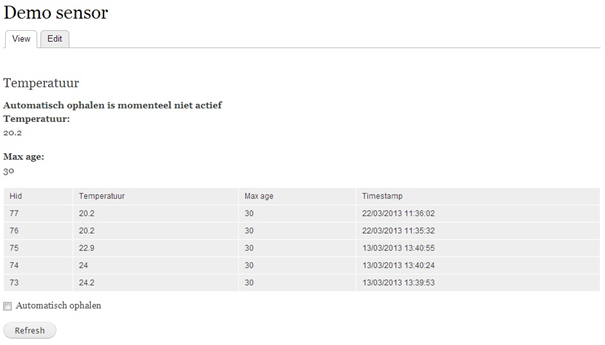
\includegraphics[width=1\textwidth]{fig/TemperatuurModuleHTTPCOAPProxy}
\vspace{-30pt}
\caption{Temperatuurmodule met HTTP/COAP-proxy}
\vspace{-10pt}
\end{figure}

\subsection{Proxy}

Als proxy werd de coap.me website gebruikt van iMinds. Deze biedt de mogelijkheid om de notificaties van een embedded device te bekijken in een browser. De website biedt ook de mogelijkheid om door te klikken naar de notificatie om die volledig te bekijken op een pagina.\\

Het is deze laatste pagina die periodiek wordt opgehaald en geparsed. De communicatie vanwege de Drupal-module bestaat dus enkel uit HTTP-communicatie, de proxy verzorgt de nodige CoAP-berichten tussen zichzelf en het embedded device.

\subsection{Achtergrondprocessen}

In een eerste fase van deze module werd er gebruik gemaakt van een formulier en werd bij het indienen van dit formulier, eerst de request uitgevoerd en dan gewacht op de response om de nieuwe pagina op te bouwen. Het spreekt voor zich dat dit geen goed oplossing is, daar de gebruiker zal moeten wachten op de pagina wanneer de communicatie traag is of misloopt, de gebruiker kan snel het idee krijgen dat er geen verbinding meer is met de website.\\

In het vorige hoofdstuk zagen we dat een mogelijke oplossing het gebruik van jQuery is. In deze situatie is jQuery echter geen goede optie, daar jQuery de databank van Drupal niet zomaar kan manipuleren. Hiervoor zouden een connectiestring, wachtwoord en dergelijke gegevens nodig zijn, en jQuery van die informatie voorzien is een grote bedreiging voor de veiligheid, bovendien zou dit een oplossing zijn met een zeer sterke koppeling, wat nooit een goed idee is.\\

De gebruikte oplossing illustreert alweer de voordelen van een open source platform met een uitgebreide community. Er is namelijk al een Background Process module gemaakt in het verleden, het zou dus zonde zijn om hier niet dankbaar gebruik van te maken. Zoals de naam suggereert, biedt de Background Process module de mogelijkheid om achtergrondprocessen op te starten. Deze draaien op de achtergrond op de server en storen dus geen andere processen zoals het opbouwen van een pagina voor de gebruiker, waardoor de gebruiker dus niet geconfronteerd wordt met lange wachttijden.\\

Sterker nog, er is ook een functie voorzien om een HTTP GET-request uit te voeren, waarbij je een callback-functie opgeeft. Wanneer er een response is, zal dus automatisch de opgegeven functie opgeroepen worden met de response als argument.

\subsection{Geschiedenis van opvragingen}

Alles is nu voorhanden om een geschiedenis bij te houden van opgevragen waarden. Het achtergrondproces kan ongestoord op de server periodiek een GET-request uitvoeren en omdat dit op de server gebeurt kunnen de waarden gemakkelijk en dynamisch toegevoegd worden aan de databank.\\

Er rest ons nu enkel nog een manier te vinden om de client op de hoogte te brengen van nieuwe waarden en hem van die waarden te voorzien.\\

Op deze manier staat het ophalen van waarden en die in de databank stoppen los van het tonen van diezelfde waarden aan de client. Dit zorgt ervoor dat een andere gebruiker evengoed ook de waarden kan bekijken, er is dus een ��n-naar-veel relatie.

\subsection{Push-strategie: node.js}

De mooiste oplossing en tevens ��n met het minste aandeel aan overhead, is een oplossing waarbij de server zelf op eigen initiatief data kan sturen naar de client. Hierbij is dan geen polling-mechanisme nodig door de client, wat de netwerkbelasting drastisch verlaagt en de verantwoordelijkheid verschuift naar de server.\\

Om een push-strategie te verwezenlijken werd een uitgebreide literatuurstudie van node.js uitgevoerd. Node.js is een javascript-library die je in staat stelt bi-directioneel verkeer te verwezenlijken. Hierbij wordt gebruik gemaakt van kanalen die worden opgezet, zo?n kanaal kan dan door beide partijen gebruikt worden.\\

Concreet zou het in de context van deze masterproef mogelijk zijn om met node.js een JavaScript-functie op te roepen bij de client op initiatief van de server.\\

Er is meermaals gepoogd dit te realiseren, maar de summiere documentatie van node.js laat op sommige vlakken te wensen over. Zo zijn we er niet in geslaagd documentatie te vinden over het opzetten van een eigen kanaal of een bestaand kanaal te gebruiken.\\

Bovendien is het nodig voor node.js om een extra server te draaien waarlangs het verkeer moet passeren. Aangezien het vaak niet mogelijk is om de shell van de webserver te gebruiken in een free-hosting omgeving, is dit een erg groot nadeel.
Er bestaan wel servers die je kan gebruiken, maar dit tegen betaling.\\

Wij, als ontwikkelaar van de module, kunnen niet verwachten dat een eindgebruiker een extra server ter beschikking heeft of dat zelfs wilt. Het is de bedoeling dat onze module zo veel mogelijk out-of-the-box bruikbaar is.\\

Vandaar dat wij geopteerd hebben geen gebruik te maken van node.js en dus ook niet van een push-strategie.

\subsection{Pull-strategie}

Aangezien een push-strategie niet of moeilijk kan gebruikt worden, hebben wij gekozen voor een pull-oplossing.\\

Uiteraard was de eerste reactie gebruik te maken van de Drupal-community en dus te zoeken in de vele modules die beschikbaar zijn. Er is tot op heden geen module geschreven door iemand anders in de Drupal-community dat ons probleem behandelt. De inspiratie voor de uiteindelijke oplossing werd wel gehaald uit een bestaande module, namelijk de Block Refresh-module.\\

Deze laatste maakt gebruik van jQuery en AJAX calls om periodiek de inhoud van een block te refreshen, waarbij je zelf de lengte van de periode kan bepalen. In jQuery loopt een timer die periodiek een JavaScript-functie oproept. In deze functie wordt dan een AJAX call uitgevoerd naar de Drupal server, die op zijn beurt een antwoord terug stuurt.\\

Hetzelfde mechanisme wordt gebruikt in onze module.
Wanneer de pagina geladen wordt bij de client, start een timer die periodiek een AJAX call uitvoert naar de Drupal server. Op de Drupal server is een AJAX callback functie gedefinieerd aan de hand van de hook hook\_menu(). Deze hook wordt gebruikt om menu items toe te voegen aan de site en om AJAX callbacks te definieren.\\

De callback-functie haalt dan de laatst toegevoegde rij op en stuurt volgende kolommen naar de client:

\begin{itemize}
\item Hid: een History-id die de opvragingen onderscheidt
\item Temperatuur: de effectieve waarde in graden Celsius.
\item Max age: De geldigheidsperiode van de waarde in seconden.
\item Timestamp: Het tijdstip van opvragen.
\end{itemize}
	
In de jQuery-functie bij de client wordt dan het opgehaalde history-id vergeleken met de hoogste history-id in de tabel op de pagina.
Als de opgehaalde waarde nieuwer is dan die op de pagina, wordt de nieuwe rij ingevoegd bovenaan de tabel op de pagina.

\section{Temperatuurmodule met native CoAP}


\chapter{Uitbreidingen} \label{uitbreidingen}

Het eindresultaat van onze module is een afgerond geheel en is dus ook bruikbaar. Er zijn echter nog enkele mogelijke uitbreidingen die wij voor ogen zagen. Deze hebben wij niet ge\"{i}mplementeerd wegens tijdsgebrek. We sommen in dit hoofdstuk enkele van deze uitbreidingen op en bespreken hoe wij ze eventueel zouden implementeren.

\section{Keuze van interval bij automatisch ophalen}
Onze huidige module voorziet een alternatieve vorm van de CoAP observe voor CoAP resources die niet observable zijn. Een gebruiker kan namelijk waarden periodiek laten ophalen, dit gebeurt
aan de hand van opeenvolgende GET requests waartussen een bepaald interval ligt. In onze module bedraagt die een hardgecodeerd aantal seconden (namelijk 5). Men zou echter de module
gebruiksvriendelijker en meer configureerbaar kunnen maken door de gebruiker het interval te laten kiezen. Dit zou gelijkaardig kunnen gebeuren aan de keuze van het polling interval, eerder
besproken in paragraaf \ref{rest}.

\section{Opvragen devices in subnetwerk met resource directory} \label{resourceDirectory}
Eerder werd al uitgelegd hoe resource discovery in zijn werk gaat (Zie paragraaf \ref{resourceDiscovery}). Men kan dit principe doortrekken op subnetwerkniveau. Wanneer op een subnetwerk een resource directory voorzien is
kunnen embedded devices er hun well-known/core's in plaatsen. De module zou dan de gebruiker een lijst kunnen presenteren die alle aanwezige devices in het subnetwerk opsomt, samen
met de aangesloten resources. Men zou ook hier weer modulair kunnen werken en de devices voorstellen als instanties van het content type CoAP device.\\

Nog een ander mogelijk alternatief dat overwogen werd is het sturen van een broadcast op het subnetwerk. Deze broadcast bevat dan een GET request die de well-known/core opvraagt
van elk embedded device in het subnetwerk. Het nadeel bij deze benadering is dat een broadcast zeer belastend is voor het subnetwerk. Bovendien is het niet de bedoeling dat als een gebruiker
ge\"{i}nteresseerd is in een ander subnetwerk, dat die belasting zomaar kan worden uitgevoerd. Wanneer men echter gebruik maakt van een resource directory kan men bovendien beslissen welke
embedded devices publiek worden gemaakt, wat de beveiliging en belasting van het subnetwerk ten goede komt.

\section{Conditional observe}

Het principe van een conditional observe is een uitbreiding van de standaard CoAP observe. Het werd mede ontwikkeld door iMinds en wordt omschreven in een aparte draft, namelijk de
CoAP Conditional Observe draft (huidig versie 3) \cite{coapConditionalObserveDraft}.\\

Een conditional observe werkt net als een gewone CoAP observe met dat verschil dat een waarde pas naar de client wordt opgestuurd wanneer de waarde aan een bepaalde voorwaarde
voldoet. Dit kan bijvoorbeeld een temperatuur zijn waarvan je pas op de hoogte wilt gesteld worden wanneer die hoger wordt dan 20 graden Celsius.
Voor de conditional observe wordt optie nummer 18 gebruikt. Deze optie moet steeds vergezeld worden van een gewone observe optie (nr. 6) aangezien deze er een extensie van is.

\begin{figure}[h!]
\centering
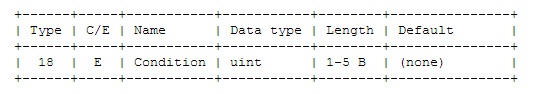
\includegraphics[width=0.8\textwidth]{fig/conditional}
\caption{Conditional observe optie (Option Delta 18)}
\end{figure}

De waarde kan vari\"{e}ren in lengte van \'{e}\'{e}n tot vijf bytes en bestaat uit de volgende onderdelen:
\begin{itemize}
\item TYPE: Beschrijft het type van de voorwaarde, bijvoorbeeld groter dan, kleiner dan, is gelijk aan,...
\item R: In een request duidt deze bit aan of de client de notificaties als CON (1) of NON (0) verkiest. In een response duidt deze bit aan of de server bereid is om in te gaan op het verzoek van de client om het betreffende soort berichten te sturen.
\item V: Deze twee bits duiden aan wat het type van de voorwaarde is (Integer, tijdsduur in seconden of float).
\item VAL: De waarde van de voorwaarde, de lengte hiervan kan vari\"{e}ren van \'{e}\'{e}n tot vier bytes.
\end{itemize}

\begin{figure}[h!]
\centering
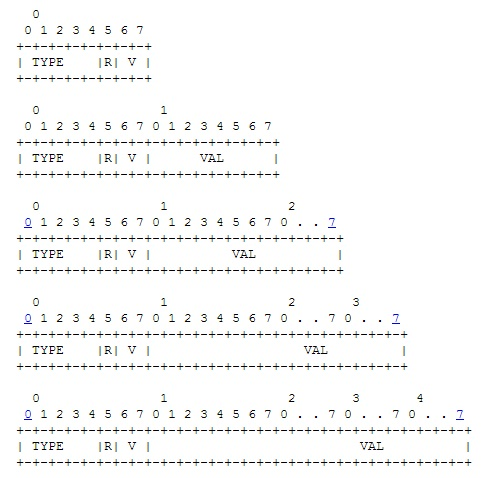
\includegraphics[width=0.8\textwidth]{fig/conditional_format}
\caption{Conditional observe optie formaat}
\end{figure}

\subsection{Keep-alive}

Men kan gebruik maken van de Keep-alive optie om er zeker van te zijn dat de client nog deel uitmaakt van de lijst van observers. Het betreft hier optie 30.\\

\begin{figure}[h!]
\centering
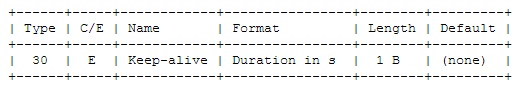
\includegraphics[width=0.8\textwidth]{fig/keep_alive}
\caption{De Keep-alive optie met Option Delta 30}
\end{figure}

Wanneer een client een Keep-alive optie meestuurt, vraagt die aan de server te bevestigen dat de client nog tot de lijst met observers behoort. En dit telkens wanneer een bepaald interval, meegegeven door de client in de optie, verstrijkt en er in dat interval geen notificaties of enkel NON-berichten ontvangen zijn. De server stuurt dan een leeg bericht op, de voorwaarde werd immers niet voldaan.

\section{Custom Entity} \label{customEntity}
We gebruiken de Entity API al voor manipulatie van content. Wat we er nog mee mogelijk is, is het ontwerpen van een eigen entity. Dit is toepasbaar op de waarden van resources. Momenteel worden waarden opgeslaan in de tabel coap\_resource\_values. Deze tabel wordt bij installatie aangemaakt en het manipuleren ervan wordt door onze eigen code afgehandeld. Als we een entity coap\_resource\_value maken, worden de waarden nog steeds in dezelfde tabel opgeslaan maar kunnen we de manipulatie ervan laten gebeuren door de functies die de Entity API aanbiedt. Een bijkomend voordeel is dat we custom views kunnen maken van entities. Gebruikers kunnen dan zelf custom views van waarden aanmaken. Een gebruiker kan dus bijvoorbeeld alle waarden van 5 mei tot 5 juni opvragen.\\
Een nuttig voorbeeld van het aanmaken van een eigen entity in code vind je in de module Model Entities \cite{modelEntities}.\\

Een bijkomende uitbreiding is het gebruik van de module Entity Reference \cite{entityReference}. Omdat we zelf een tabel cre\"{e}eren zonder aan Drupal te zeggen dat deze een speciale betekenis heeft, staan we zelf in voor de visualitatie van de waarden. Maar door een eigen entity te maken kunnen we de waarden weergeven door gebruik te maken van een nieuw veld dat ge\"{i}troduceerd wordt door de Entity Reference-module.

\section{Interface Description}
Het attribuut if (interface description) van het CoRE Link Format kan info bevatten over welke methodes deze resource ondersteund. Momenteel wordt deze info opgeslaan maar nog niet gebruikt. Deze informatie kan gebruikt worden om de methodes (GET, PUT, POST en DELETE) niet voor alle resources beschikbaar te laten zijn. De verschillende waarden en hun betekenis die het attribuut kan aannemen vind je in de CoRE Interfaces draft \cite{coreInterfaces}.

\section{View Modes}
De content die we aanbieden wordt op elke pagina op dezelfde manier getoond. Door gebruik te maken van view modes kunnen we hier verandering in brengen. Wanneer content van het type coap\_resource getoond wordt, kan je er verschillende functies op uitvoeren en zie je een historytabel. Maar soms zou het handig zijn als je enkel de historytabel ziet. Een complete tutorial met uitleg vind je online \cite{viewMode}.

\section{Configuratie op maat} \label{configuratie}
Bij installatie wordt een pagina voor configuratie voorzien. Deze kan je bereiken door eerst op 'Configuration' te klikken en dan op 'CoAP resource settings'. Enige configuratieinstellingen komen hier te staan. Om de pagina die getoond wordt aan passen moet je de functie coap\_resource\_admin\_settings() in coap\_resource.module aanpassen.
\begin{figure}[h!]
\vspace{10pt}
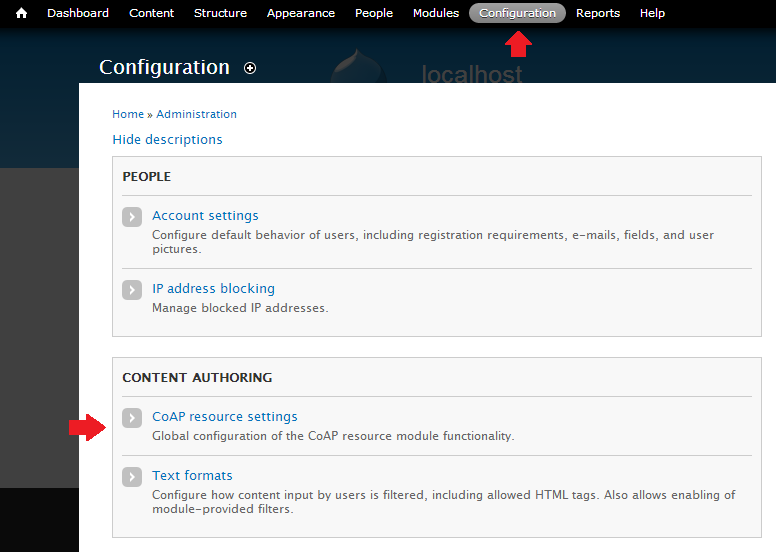
\includegraphics[width=1\textwidth]{fig/Configuratie}
\vspace{-30pt}
\caption{Navigatie naar de configuratiepagina}
\vspace{-10pt}
\end{figure}

\section{Help}
Een standaard hulppagina is voorzien, deze kan opgevuld worden met de handleiding.
\begin{figure}[h!]
\vspace{10pt}
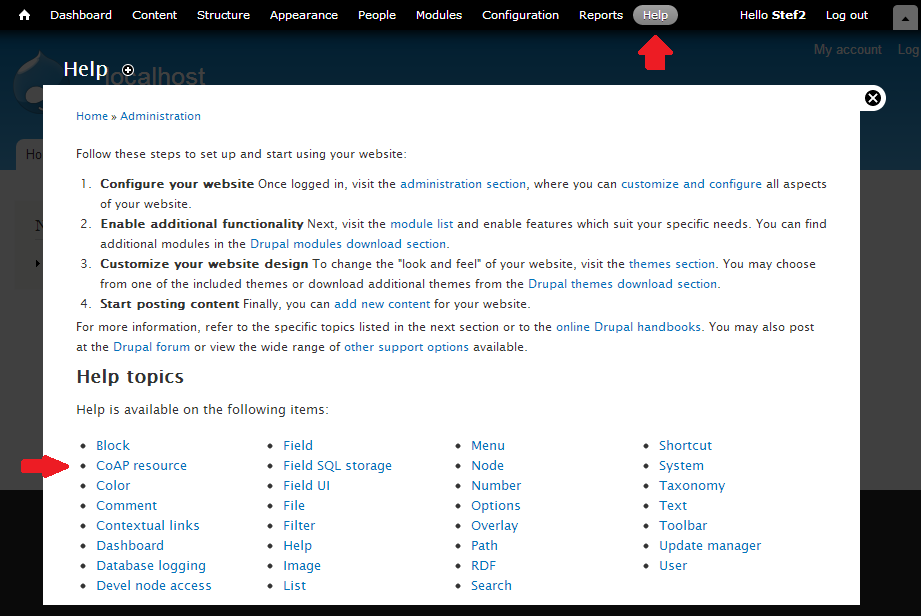
\includegraphics[width=1\textwidth]{fig/Help}
\vspace{-30pt}
\caption{Navigatie naar de hulppagina}
\vspace{-10pt}
\end{figure}

Er kan ook gebruik gemaakt worden van de Advanced Helpmodule \cite{advancedHelp}. Wanneer deze module ge\"{e}nabled is, kan je helppagina's opslaan in HTML-formaat en deze in je moduledirectory zetten. Deze module maakt ook het gebruik van popups mogelijk en laat de administrator van de website beslissen voor wie de hulp beschikbaar moet zijn. We laten het aan de lezer over om alle mogelijkheden van deze module te bekijken.

\section{DNS}
Het programma werkt enkel met IP-adressen. Door gebruik te maken van de PHP-functies gethostbyaddr(string \$ip\_addr)\cite{hostByAddr} en gethostbyname(string \$hostname)\cite{{hostByName}} kunnen hostnamen gebruikt worden i.p.v. hun respectievelijk IP-adres.

\section{Block Options} \label{unsupportedBlockOptions}
Voor optie 28 (Size) en 27 (Block1) bieden we nog geen ondersteuning, momenteel worden ze genegeerd. Block1 hebben we reeds besproken in \ref{blocks}. De Size-optie wordt voor meerdere dingen gebruikt, maar ze hebben allemaal een verband met een schatting van de grootte van de resource representatie:
\begin{itemize}
\item In een request: om aan de server te vragen of hij een schatting meestuurt met zijn response. Hier moet als waarde 0 gebruikt worden.
\item In een response met een Block2-optie: om de schatting van de server aan te geven.
\item In een response met een Block1-optie: om de schatting van de client aan te geven.
\end{itemize}
De client of server kan aan de hand van de schatting beslissen om grotere of kleinere blocks door te sturen. Deze optie is niet verplicht te ondersteunen dus moet er rekening gehouden worden met dat de server of client deze optie negeert.

\section{Anonieme gebruikers}
Momenteel worden anonieme gebruikers niet meer ondersteund. Er is wel een analyse uitgevoerd hoe ze best ge\"{i}mplementeerd worden. Voor anonieme gebruikers is het beter om zelf geen gegevens naar de databank te schrijven. Dit om ervoor te zorgen dat de databank niet geflood wordt.

Anonieme gebruikers hebben als User ID (uid)\nomenclature{uid}{User ID} het getal 0. Anders dan gewone gebruikers die een uniek uid hebben kan je anonieme gebruikers hier niet op onderscheiden. Gebruikers hebben ook een Session ID (sid)\nomenclature{sid}{Session ID} dat wel uniek is voor alle gebruikers. Nu moeten we de gegevens van de anonieme gebruiker bijhouden op een plaats die overal toegankelijk is maar dit mag niet de databank zijn. Daarom wordt er gebruik gemaakt van de sessievariabele \cite{sessionVariable} \$\_SESSION. Deze variabele is een PHP-tabel en het ligt voor de hand deze te indexeren op de sid. Alle gegevens worden nu best opgeslaan en aangesproken op volgende manier: \$\_SESSION[\$sid] met \$sid een variabele die de sid van de gebruiker bevat. 

% appendices
\appendix

% hier worden de appendices ingevoegd (\includes)


%dit moet nog binnen dutch komen, anders staat er Bibliography
\begin{thebibliography}{99}

%referenties zijn typisch in het Engels
\selectlanguage{english}
 
%\bibitem{leos2000} K. Steenbergen, F. Janssen, J. Wellen, R. Smets, T. Koonen,
%\newblock ``Fast wavelength-and-time slot routing in hybrid fiber-access
%networks for IP-based services'',
%\newblock in {\em IEEE LEOS Symposium}, Delft, The Netherlands,
%October~2000.
 
%\bibitem{2-BIT} K. Nichols, V. Jacobson, L. Zhang,
%\newblock ``A two-bit differentiated services architecture for the
%Internet'',
%\newblock {\em IETF RFC~2638},
%July~1999.                                       

%\bibitem{omniorb} http://www.omniorb.org

\bibitem{beginDrupal} Tomlinson T. (Juni, 2010) {\em Beginning Drupal 7.} APress.

\bibitem{proDrupal} Travis B. (Februari, 2011) {\em Pro Drupal 7 for Windows developers.} APress.

\bibitem{drupalDefGuide} Melançon B., Luisi J., Négyesi K., Anderson G., Somers B., Corlosquet S., Freudenberg S., Lauer M., Charlevale E., Lorétan F., Nordin D., Szrama R., Stewart S., Strawn J., Travis B., Hakimzadeh D., Scavarda A., Albala A., Micka A., Douglass R., Monks R., Scholten R., Wolanin P., VanValkenburgh K., Stout G., Dolin K, Mars F., Boyer S., Gifford M., Sarahe C. (2011). {\em The Definite Guide to Drupal 7.} APress.

\bibitem{formApi} http://api.drupal.org/api/drupal/developer!topics!forms\_api\_reference.html/7, 18 februari 2013

\bibitem{yahooWeatherApi} http://developer.yahoo.com/weather/, 18 februari 2013

\bibitem{installHook} http://api.drupal.org/api/drupal/modules!system!system.api.php/function/hook\_install/7, 18 februari 2013

\bibitem{schemaHook} http://api.drupal.org/api/drupal/modules!system!system.api.php/function/hook\_schema/7, 18 februari 2013

\bibitem{enableHook} http://api.drupal.org/api/drupal/modules!system!system.api.php/function/hook\_enable/7, 18 februari 2013

\bibitem{backgroundProcessModule} http://drupal.org/project/background\_process, 19 februari 2013

\bibitem{progressModule} http://drupal.org/project/progress, 19 februari 2013

\bibitem{crossDomainProblem} http://stackoverflow.com/questions/12683530/origin-http-localhost-is-not-allowed-by-access-control-allow-origin, 17 maart 2013

\bibitem{entityApiModule} http://drupal.org/project/entity, 24 april 2013

\bibitem{addTemplate} http://www.metachunk.com/blog/adding-module-path-drupal-7-theme-registry, 14 mei 2013

\bibitem{preprocessHook} http://api.drupal.org/api/drupal/modules!system!theme.api.php/function/hook\_preprocess\_HOOK/7, 14 mei 2013

\bibitem{coapDraft} http://datatracker.ietf.org/doc/draft-ietf-core-coap/, 21 mei 2013

\bibitem{coapObserveDraft} http://datatracker.ietf.org/doc/draft-ietf-core-observe/, 21 mei 2013

\bibitem{coapConditionalObserveDraft} http://tools.ietf.org/html/draft-li-core-conditional-observe-03, 21 mei 2013

\bibitem{coapDiscovery} http://tools.ietf.org/html/rfc6690, 21 mei 2013

\bibitem{blockwiseTransfer} http://tools.ietf.org/html/draft-ietf-core-block-11, 21 mei 2013

\bibitem{coreInterfaces} http://tools.ietf.org/html/draft-shelby-core-interfaces-05, 21 mei 2013

\bibitem{copper} https://addons.mozilla.org/en-US/firefox/addon/copper-270430/, 21 mei 2013

\bibitem{entities} http://drupal.org/node/1261744

\bibitem{wireshark} http://www.wireshark.org

\end{thebibliography}

\selectlanguage{dutch}

\backmatter

% eventueel: lijst van uren en tabellen
\listoffigures
%\listoftables

% lege pagina (!!)

% kaft

\end{document}
